\documentclass[a4paper,12pt]{article} % тип документа


\usepackage[T2A]{fontenc} % кодировка
\usepackage[utf8]{inputenc} % кодировка исходного текста
\usepackage[english,russian]{babel} % локализация и переносы

% colors
\usepackage[dvipsnames,table,xcdraw]{xcolor}          
\definecolor{light-blue}{rgb}{0.8,0.85,1}


%symbols
\usepackage{upgreek}
\usepackage{amsmath,amsfonts,amssymb,amsthm,mathtools} %math
% теоремы
\theoremstyle{plain}
\newtheorem{definition}{Определение}[section] 
\newtheorem{theorem}{Теорема}
\newtheorem{example}{Пример}
\numberwithin{equation}{section}



% гиперссылки:
\usepackage{hyperref}
\definecolor{darkblue}{HTML}{0000A0}
\definecolor{linkcolor}{HTML}{0000FF}
\hypersetup{pdfstartview=FitH, citecolor=linkcolor, linkcolor=darkblue,urlcolor=red, colorlinks=true}


% графика:
\usepackage{graphics}
\graphicspath{{pic/}}
\DeclareGraphicsExtensions{.pdf,.png,.jpg, .eps}
\usepackage{caption} % а что без этого летит? (забыл)
\usepackage[section,above,below]{placeins} % управление плавающими объектами (?)
\usepackage{floatflt}
\usepackage{framed}



% работа с таблицами (?)
\usepackage{multirow}
\newcommand{\specialcell}[2][c]{%
	\begin{tabular}[#1]{@{}c@{}}#2\end{tabular}} % перенос строки в ячейке таблицы при пакете multirow


\newcommand{\comment}[1]{} % for multiline comments

% defining red box
\newsavebox{\selvestebox}
\newenvironment{colbox}[1]
{\newcommand\colboxcolor{#1}%
	\begin{lrbox}{\selvestebox}%
		\begin{minipage}{\dimexpr\columnwidth-2\fboxsep\relax}}
		{\end{minipage}\end{lrbox}%
	\begin{center}
		\colorbox[HTML]{\colboxcolor}{\usebox{\selvestebox}}
\end{center}}

% предметный указатель и библиография
\usepackage{makeidx}
\makeindex
\usepackage[nottoc]{tocbibind}

% разметка и стиль (???)
\usepackage[left=2cm, right=2cm, top=2cm, bottom=2cm]{geometry}
\usepackage{fancyhdr}
\pagestyle{fancy}
\fancyhead[L]{\rightmark}
%\lhead{ краткое название}
\chead{}
\rhead{\thepage}
\cfoot{} % get rid of the page number 
\renewcommand{\headrulewidth}{1pt}
\renewcommand{\footrulewidth}{0pt}
\usepackage{indentfirst}

\usepackage{framed}
\usepackage{fancyvrb} %for fraim aroun verbatim
 % основная шапка


\author{Юрий Голубев\\ yura.winter@gmail.com }
\title{статистическая физика}
\date{\today}

\usepackage{graphicx} 
\usepackage{float} 

\newcommand{\parder}[2]{\frac{\partial {#1}}{\partial {#2}}}

\begin{document}
\maketitle

\begin{abstract}
Задачи по статической физике.
\end{abstract}
%%%%%%%%%%%%%%%%%%%%%%%%%%%%%%%%%%%%%%%%%%%%%%%%%%%%%%%%%%%%%%	
\tableofcontents

\section*{Предисловие}
\addcontentsline{toc}{section}{Предисловие}


Задачи по статистической физике.






\clearpage
\part{упражнения}


\begin{task}\textbf{1}

$ N $ молекул идеального газа в объеме $ V $. 
Определить вероятность того, что в объеме $v < V$ находится $ n $ молекул. Получить приближенное выражение, когда  $v \ll V $. 
Найти среднее число частиц $\overline{n}$ в объеме $ v $, его среднюю абсолютную и относительную флуктуации.  


Вероятность попадания ровно одной молекулы в объем $ V$ равна $ p=\frac{v}{V}$. 
Поэтому вероятность попадания ровно $n$ молекул в объем $V$ равна 
\[ p^n (1-p)^{N-n} \]
В объем сосуда могут попасть разные молекулы, всего нужных нам комбинаций:
\[ C_N^n =\frac{N!}{n!(N-n)!}\]
Поэтому искомая вероятность:
\[ P(n)=\frac{N!}{n!(N-n)!}p^n (1-p)^{N-n} \]

Поищем предел $v \ll V$,  для него можно считать, что $ p\ll 1, n\gg 1$, также можно предположить, что $ np=\lambda$, которое конечно и не слишком мало, не слишком велико.
В таком случае имеется известный предел - распределение становится распределением Пуассона.
\[ P(n)=\frac{\lambda^k}{k!}e^{-\lambda}=
\frac{np^k}{k!}e^{-np}\]

Среднее значение $\overline{n}$ можно найти, зная, что вероятность попадания в данный объем линейно зависит от объема:
\[ \overline{n}=\frac{v}{V}N=Np \]

Или то же самое, если записать по определению среднего:
$$
\overline{n^{k}}=\sum_{n=0}^{\infty} C_{N}^{n} n^{k} p^{n} q^{N-n}=\left(p \frac{\partial}{\partial p}\right)^{k} \sum_{n=0}^{\infty} C_{N}^{n} p^{n} q^{N-n}=\left(p \frac{\partial}{\partial p}\right)^{k}(p+q)^{N}
$$
Тогда
$$
\bar{n}=\left(p \frac{\partial}{\partial p}\right)(p+q)^{N}=p N(p+q)^{N-1}=p N
$$
\[
\overline{n^{2}}=\left(p \frac{\partial}{\partial p}\right)^{2}(p+q)^{N}=p N+p N p(N-1)=p N[1+p(N-1)] 
\]
и дисперсия  $\sigma_{n}^{2}=\overline{n^{2}}-\bar{n}^{2}=p N[1+p N-p-p N]=N p q$

А относительная флуктуация равна:
\[ \frac{\sqrt{D n}}{\overline{n}}=\frac{\sqrt{Npq}}{Np}=\sqrt{\frac{q}{Np}}. \]

Пусть $ v\ll V, \overline{n}\gg 1 $

$$
P_{u}(v)=P(n, \lambda)=\frac{\lambda^{n} e^{\lambda}}{n !}
$$
Используя формулу Стирлинга, получаем:
$$
P_{n}(\sigma) \approx \frac{e^{-\lambda}}{\sqrt{2 \pi n}}\left(\frac{e \lambda}{n}\right)^{n}=\frac{1}{\sqrt{2 \pi n}} 
\operatorname{exp}\left(-\lambda+n+n \ln \left(\frac{\lambda}{n}\right)\right)
$$

Просто преобразуем $ P(v)$, введя $ x\equiv \lambda -n$, тогда логарифм раскрывается так: $\ln \frac{\lambda}{n}=\ln \left(\frac{n+x}{n}\right)=\ln \left(1+\frac{x}{n}\right) \approx \frac{x}{n}-\frac{1}{2}\left(\frac{x}{n}\right)^{2}$
%
$$
P_{4}(v)=\frac{1}{\sqrt{2 \pi n}} \operatorname{exp}\left(-x+x-\frac{1}{2} \frac{x^{2}}{n}\right)=
P_{4}(v)=\frac{1}{\sqrt{2 \pi n}} \operatorname{exp}\left(\frac{(\lambda - n)^2}{2\lambda}\right)
$$
это распределение Гаусса



\end{task}


\begin{task}\textbf{2}

Вычислить $ C_p-C_v$ в  переменных $ V, T $ и $ P, T$. 

Определить $ C_p-C_v$ для больцмановского газа,
газа Ван-дер-Ваальса, ферми и бозе-газа и черного излучения.

Первое начало термодинамики:
$$
\delta Q=d U+p d V,
$$
поэтому:
$$
C_{V}=\left(\frac{\partial U}{\partial T}\right)_{V}
$$
Считая внутреннюю энергию $U$ функцией температуры и объема, можем записать
\begin{equation}\label{1}
C_{p}=C_{V}+\left[\left(\frac{\partial U}{\partial V}\right)_{T}+p\right]\left(\frac{\partial V}{\partial T}\right)_{p}
\end{equation}
Выражение в квадратных скобках в правой части легко вычислить, воспользовавшись фундаментальным равенством Гиббса:
$$
T d S=d U+p d V
$$
Имеем:
$$
T\left(\frac{\partial S}{\partial V}\right)_{T}=\left(\frac{\partial U}{\partial V}\right)_{T}+p
$$
Далее, из соотношения
$$
d F=-S d T-p d V
$$
следует равенство
$$
\left(\frac{\partial S}{\partial V}\right)_{T}=\left(\frac{\partial p}{\partial T}\right)_{V}
$$
Поэтому
$$
\left(\frac{\partial U}{\partial V}\right)_{T}+p=T\left(\frac{\partial p}{\partial T}\right)_{V}
$$
Теперь с помощью соотношения \ref{1} получаем
$$
C_{p}-C_{V}=T\left(\frac{\partial p}{\partial T}\right)_{V}\left(\frac{\partial V}{\partial T}\right)_{P}
$$

И используя 
\[ \left(\frac{\partial z}{\partial x}\right)_{y}\left(\frac{\partial x}{\partial y}\right)_{z}\left(\frac{\partial y}{\partial z}\right)_{x}=-1, \]
запишем:
\begin{equation}\label{2}
C_{p}-C_{V}=
-T\left(\frac{\partial V}{\partial T}\right)_{p}^{2}\left(\frac{\partial V}{\partial p}\right)_{T}^{-1}
\end{equation}
или
\begin{equation}\label{3}
C_{p}-C_{V}=
-T\left(\frac{\partial p}{\partial T}\right)_{V}^{2}\left(\frac{\partial p}{\partial V}\right)_{T}^{-1}
\end{equation}


Теперь применим эти формулы для больцмановского газа, для которого $ pV=\nu RT $, имеем:
\[ \left(\frac{\partial V}{\partial T}\right)_{p}=\frac{\nu R}{p} \]
\[\left(\frac{\partial V}{\partial p}\right)_{T} =-\frac{\nu RT}{p^2} \]
Поэтому при подстановке в \ref{2} много множителей сокращаются и имеем:
\[ C_p-C_V=\nu R \]

Теперь применим эти формулы для газа Ван-дер-Ваальса, для которого $ \left(p+\frac{a\nu^2}{V^{2}}\right)\left(\frac{V}{\nu}-b\right)=R T$. 
Будем для просто ты считать, что $\nu=1$. 
И также тут разумнее подставлять все в \ref{3}
Получаем:
\[ \left(\frac{\partial p}{\partial T}\right)_{V}=\frac{R}{V-b} \]
\[ \left(\frac{\partial p}{\partial V}\right)_{T}=-\frac{RT}{(V-b)^2}+\frac{2a}{V^3} \]
Таким образом, подставляем и получаем:
\[ C_p-C_V=\frac{TR}{T-\frac{2a}{V^3}\left(V-b\right)^2} \]


Теперь применим эти формулы для фермии и бозе-газа, для которых $ \frac{pV}{NT}=1\pm \alpha\left(\frac{T_0}{T}\right)^{3/2}.$ Подставим, посчитаем производные, придем к ответу:
\[ C_p-C_V =\frac{N(\alpha T_0^{3/2}N \mp 2 T^{3/2} V)^2 }{\pm 8 \alpha T_0^{3/2} N T^{3/2}+4 T^3 V^2 } \] 





Теперь применим эти формулы для черного излучения. Для такого: $ p=\frac{a}{3} T^4$. Поэтому для него $ C_p-C_V\rightarrow\infty $
 


\end{task}


\begin{task}\textbf{3}

Вычислить число состояний одноатомного больцмановского газа.

Пусть имеется частиц $N$ частиц в объеме $V$. 
Поступательное движение частиц всегда квазиклассично. 
В классической механике состояние системы характеризуется точкой в $6 N-$ мерном фазовом пространстве
\begin{equation}\label{ss}
\alpha=
\left(\mathbf{r}_{1}, \mathbf{p}_{1}, \mathbf{r}_{2}, \mathbf{p}_{2}, \ldots, \mathbf{r}_{\mathbf{N}}, \mathbf{p}_{\mathbf{N}}\right)
\end{equation}
Число точек в элементе 6 -мерного фазового объема $d r^{3} d p^{3}$ согласно правилу Бора-Зоммерфельда равно отношению этого объема к $(2 \pi \hbar)^{3} .$ 
Обобщение этого правила на случай $N$ одинаковых частиц дает дифференциал числа состояний
$$
d \Gamma_{\alpha}=\frac{1}{N !} \prod_{i=1}^{N} \frac{d^{3} r_{i} d^{3} p_{i}}{(2 \pi \hbar)^{3}}
$$
Произведение дифференциалов поделено на $N !$ для того, чтобы все конфигурации, положения частиц в $6 N$ -мерном фазовом пространстве, 
отличающиеся друг от друга лишь перестановками тождествен ных частиц, учитывались только один раз. 
С помощью \ref{ss} произвольная сумма по состояниям может быть представлена в форме интеграла
$$
\sum_{\alpha} F_{\alpha}=\int d \Gamma_{\alpha} F_{\alpha}
$$


Полное число состоя ний - число точек в $6 N$ -мерном пространстве с энерг ией
$$
E_{\alpha}=\sum_{i=1}^{N} \frac{p_{i}^{2}}{2 m}
$$
А так как $ \Gamma(E)=\sum_{\alpha} \theta\left(E-E_{\alpha}\right)$, то в интервале между 0 и $E$ выражается интегралом:
$$
\Gamma(E)=\int d \Gamma_{\alpha} \theta\left(E-E_{\alpha}\right)=\frac{1}{N !} \int \prod_{i=1}^{N} \frac{d^{3} r_{i} d^{3} p_{i}}{(2 \pi \hbar)^{3}} \theta\left(E-\sum_{i=1}^{N} \frac{p_{i}^{2}}{2 m}\right)
$$
Интегрирование по пространственным координатам каждой частицы дает объем $V,$ и с учетом формулы Стильтьеса получаем
$$
\begin{aligned}
\Gamma(E) &=\left(\frac{V e}{N(2 \pi \hbar)^{3}}\right)^{N} J_{3 N}(E) \\
J_{3 N}(E) &=\int \prod_{i=1}^{N} d^{3} p_{i} \theta\left(E-\sum_{i=1}^{N} \frac{p_{i}^{2}}{2 m}\right) - \text{объем 3n мерного шара радиусом p}
\end{aligned}
$$
%
\[ V_{3N}(p)= \frac{\pi^{3N/2}}{\Gamma (\frac{3N}{2}+1)}p^n \approx \left( \frac{2 e \pi p^2}{3N}\right)^{3N/2}  \]
%
Тогда:
\[ \Gamma(E)= \left( \frac{Ve}{N (2\pi\hbar)^3}\right)^N \left(\frac{4e\pi m E^2}{3N}\right)^{3N/2}\]



\end{task}


\begin{task}\textbf{4}

Вычислить число состояний системы $ N $ независимых спинов 1/2.


Систему $N$ спинов $S=\frac{1}{2},$ находящихся в магнит ном поле $B,$ будем описывать гамильтонианом
$$
H=-2 \mu B \sum_{i=1}^{N}\left(s_{i}^{z}-\frac{1}{2}\right)
$$
Энергия одного спина в магнитном поле, равная $-2 \mu B s^{z}\left(s^{z}=\pm \frac{1}{2}\right),$ сдвинута на константу, чтобы минимальная энергия была равна нулю. 
Если $(\vec{N}-M)$ спинов находятся в основном состоя нии $\left(s^{z}=1 / 2\right),$ а $M$ спинов $-$ в возбужденном $(s^{z}=-1 / 2),$ то система имеет энергию $E=M \Delta E,$ где $\Delta E=2 \mu B .$ 
Такая энергия может быть полу чена числом способов, равным:
\begin{equation}\label{ll}
\Delta \Gamma_{M}=\frac{N !}{M !(N-M) !}
\end{equation}

Это и есть наше требуемое число состояний.

При больших значениях аргумента по формуле Стирлинга факториал приближенно равен
$$
N ! \approx(N / e)^{N}
$$
и выражение \ref{ll} принимает вид
$$
\Delta \Gamma=\left(\frac{N}{e}\right)^{N}\left(\frac{e}{M}\right)^{M}\left(\frac{e}{N-M}\right)^{N-M}=\frac{N^{N}}{M^{M}(N-M)^{N-M}}
$$

Из этого выражения можно найти энтропию и другие характеристики, но о них не спрашивается, так что задача решена.


\end{task}


\begin{task}\textbf{5}

Вычислить число состояний системы $ N $ одинаковых независимых осцилляторов.


За вычетом энергии нулевых колебаний энергия системы равна
$$
E=\Delta E \sum_{i=1}^{N} n_{i}, \quad \Delta E=\hbar \omega
$$
где $n_{i}$ - номер возбуждения $i$ -того осциллятора. Это значение энергии может быть получено числом способов, которое следует из комбинаторики
$$
\Gamma=\frac{(N+M-1) !}{(N-1) ! M !} \approx \frac{(N+M)^{N+M}}{N^{N} M^{M}}
$$




\end{task}


\begin{task}\textbf{6}

Получить выражения для неравновесной энтропии ферми- и бозе-газов



Вероятность произвольного состояния:
$$
w_{\alpha}=w\left(т_{p_{1}}\right) \cdot w\left(u_{p_{2}}\right) w\left(u_{p_{3}}\right)\cdot ...
$$


$$
S=-\sum_{x} w_{\alpha} ln w_{\alpha}=-\sum_{n_{p_1}}\sum_{n_{p_2}}\sum_{n_{p_3}}\ldots 
(w\left(u_{p_{2}}\right) w\left(u_{p_{3}}\right)\cdot ...)
(\ln w(n_{p_1})+\ln w(n_{p_2})+... )
$$

\[ S=-\sum_{n_{p_1}}
w(n_{p_1}) \ln w(n_{p_1}) +\ldots \]



Для ферми газа:$ n_p=\{ 0, 1\} $

\[ -\sum_{n_p}w(n_{p}) \ln w(n_{p})=
-w(n_{p_1}) \ln w(n_{p_1})+
w(n_{p_0}) \ln w(n_{p_0})    \]


среднее число частиц с импульсом $ p: \overline{n_p}=\sum_{n_p}w(n_p) n_p =w (1_p)$
%
\[ w(0_p)=1-\overline{n_p} \]
%
поэтому:
\[ -\sum_{n_p}w(n_p)\ln w(n_p) = -(1-\overline{n_p})\ln (1-\overline{n_p}) - \overline{n_p} \ln \overline{n_p}\]


В итоге энтропия для ферми газа равна:
\[ S_F=-\sum_{p}\Big(
(1-\overline{n_p}) \ln (1-\overline{n_p})+\overline{n_p} \ln \overline{n_p}\Big) \]



Теперь то же для бозе-газа. Для него $ n_p\in \{0, ... \infty\} $


Сумма $ \Big[-\sum_{n_p} w(n_p) \ln (n_p)\Big]$ принимает максимальное значение при заданном $ \overline{n_p}$ при условии на функцию Лагранжа:
\[ L= -\sum_{n_p} w(n_p) \ln (n_p) -\lambda_1 \sum_n n w(n) - \lambda_2 \sum_n w(n)\]

$$
\frac{\partial L}{\partial w(n)}=-\ln w(n)-1 -\lambda_1 n - \lambda_2
$$
$$
w(n)=\exp\left(-1-\lambda_{1} n-\lambda_{2}\right)
$$

$$
\sum w_{n}=1 \Rightarrow \exp \left(-1-\lambda_{1} n-\lambda_{2}\right)=1
$$
$$\sum
\exp \left(-1-\lambda_{2}\right) \sum_{n} \exp (-\lambda_1 n)=1
$$

$$
\sum_{n} \operatorname{exp}\left(-\lambda_{1} n\right)=
\frac{1}{1-e^{-\lambda_{1}}} \Rightarrow \operatorname{exp}\left(-1-\lambda_{2}\right)=1-e^{-\lambda_{1}}
$$


$$
\bar{n}=\sum_{n} w(n) n=\exp \left(-1-\lambda_{2}\right) \sum_{n} n 
\exp \left(-\lambda_{1} n\right)=\exp \left(-1-\lambda_{2}\right)
$$
\[ \left(-\frac{d}{d \lambda_1} \sum_{n} \exp \left(-\lambda_{1} n\right)\right)=-\exp \left(-1-\lambda_{2}\right) \frac{d}{d \lambda_{1}} \frac{1}{1-e^{-\lambda_{1}}} \]
%
\[ \bar{n}=\frac{1}{e^{\lambda_{1}}-1 } \]
\[ e^{-\lambda_{1}}=\frac{\bar{n}}{\bar{n}+1} \]




Поэтому после преобразований получаем:
$$
w(n)=\frac{1}{\bar{n}+1}
\left(\frac{\bar{n}}{\bar{n}+1}\right)^{n}
$$


\begin{multline}
S=-\sum_{n} w(n) \ln w(n)=\sum_{n} w(n)\left(\lambda_{1} n+\lambda_{2}+1\right) =\\
= \sum_{n} w_{n}\left(\lambda_{2}+1\right)+\sum_{n} n w_{n} \lambda_{1}=\left(\lambda_{2}+1\right)+\bar{n} \lambda_{1}=\\
=(\bar{n}+1) \ln (\bar{n}+1)-\bar{n} \ln \bar{n}
\end{multline}

В итоге:
$$
S=\sum_{p}\left[\left(1+\bar{n}_{p}\right) \ln \left(1+\bar{n}_{p}\right)-n_{p} \ln \overline{n_{p}}\right]
$$



\end{task}


\begin{task}\textbf{7}

Вычислить основные термодинамические величины ферми- и бозе-газов при $T=0$


Для ферми газа:

\[	N=\sum_{p}N_{p} \approx \frac{2 V}{(2 \pi \hbar)^{3}} \int_{0}^{p_{F}} n_{p} 4 \pi p^{2} dp=\frac{V}{3 \pi^{2} \hbar^{3}} p_{F}^{3} \]

\[ 
E=\sum_{p}\left(E_{p} n_{p}\right) \approx \frac{2 V 4 \pi}{(2 \pi \hbar)^{3} 2 m} \int_{0}^{p_{F}} p^{4} d(p)=\frac{3}{5} N E_{F}  \]

Давление находится по известной формуле:
\[ 	P=-\parder{E}{V}=
-\frac{\partial}{\partial V}\left(\frac{3}{10}\left(3 \pi^{2}\right)^{\frac{2}{3}} \frac{\hbar^{2}}{m} \frac{N^{\frac{5}{3}}}{V^{\frac{2}{3}}}\right)=
\frac{1}{5}\left(3 \pi^{2}\right)^{\frac{2}{3}} \frac{\hbar^{2}}{m} n^{\frac{5}{3}}=
\frac{2}{5} n E_{F} \]




\end{task}


\begin{task} \textbf{8}



Из функционала Гинзбурга–Ландау получить выражение для плотности тока в магнитном поле, получить уравнение Лондонов и квантование магнитного потока в сверхпроводящем кольце.









Потенциал Гиббса во внешнем магнитном поле $\mathrm{H}_{0}$ вблизи $T_{c}$ можно представить в виде разложения по малому параметру $\Psi$ :



\[ 
G_{s h}=
G_{n}
+
\alpha|\Psi|^{2}
+
\frac{\beta}{2}|\Psi|^{4}
+
\frac{1}{4 m}\left|\left(\hat{\mathbf{p}}-\frac{2 e}{c} \mathbf{A}\right) \Psi\right|^{2}
+
\frac{(\operatorname{rot} \mathbf{A})^{2}}{8 \pi}
-
\frac{\operatorname{rot} \mathbf{A} \cdot \mathbf{H}_{0}}{4 \pi} 
\]


\[ 	
\operatorname{rot} \mathbf{A} \equiv \mathbf{B},
\qquad
\hat{\mathbf{p}}=-i \hbar \nabla 
\]


$G_{n}-$ плотность свободной энергии в нормальном состоянии. 







Найдем, при каких значениях $\Psi$ и А свободная энергия Гиббса
$$
\begin{array}{c}
	\mathcal{G}_{s H}
	=
	\mathcal{G}_{n}
	+
	\int d V \left[
	\alpha|\Psi|^{2}
	+
	\frac{\beta}{2}|\Psi|^{4}
	+
	\frac{1}{4 m}\left|-i \hbar \nabla \Psi-\frac{2 e}{c} \mathbf{A} \Psi\right|^{2}
	+
	\frac{(\operatorname{rot} \mathbf{A})^{2}}{8 \pi}
	-
	\frac{\operatorname{rot} \mathbf{A} \cdot \mathbf{H}_{0}}{4 \pi}\right]
\end{array}
$$
имеет минимум?






Первое условие минимума
$$
\delta_{\Psi^{*}} \mathcal{G}_{s H}=0
$$


Вычислим его:
$$
\begin{array}{c}
	\delta_{\Psi^{*}} \mathcal{G}_{s H}
	=
	\int d V\left[
	\alpha \Psi \delta \Psi^{*}
	+
	\beta \Psi|\Psi|^{2} \delta \Psi^{*}
	+
	\frac{1}{4 m}
	\left(i \hbar \nabla \delta \Psi^{*}
	-
	\frac{2 e}{c} \mathbf{A} \delta \Psi^{*}\right)
	\left(-i \hbar \nabla \Psi-\frac{2 e}{c} \mathbf{A} \Psi\right)
	\right]
\end{array}
$$
Подчеркнем, что действие оператора $\nabla$ ограничено соответствующими круглыми скобками. 


Введем обозначение
$$
\mathbf{p}=\left(-i \hbar \nabla-\frac{2 e}{c} \mathbf{A}\right)
$$

Тогда последнее слагаемое перепишется в виде
$$
\int d V \frac{1}{4 m}\left(i \hbar \nabla \delta \Psi^{*}-\frac{2 e}{c} \mathbf{A} \delta \Psi^{*}\right)(\mathbf{p} \Psi)
$$






Преобразуем выражение:
$$
\int d V\left(\nabla \delta \Psi^{*}\right)(\mathbf{p} \Psi)
=
\int d V\left(\nabla \delta \Psi^{*}(\mathbf{p} \Psi)\right)
-
\int d V \delta \Psi^{*} \nabla(\mathbf{p} \Psi)
$$





Первый интеграл преобразуем в интеграл по поверхности сверхпроводника
$$
\int d V \nabla\left(\delta \Psi^{*}(\mathbf{p} \Psi)\right)
=
\oint d \mathbf{S} \delta \Psi^{*}(\mathbf{p} \Psi)
$$


Поэтому в вариации с точностью до поверхностного члена выше можно сделать замену
$$
\left(\nabla \delta \Psi^{*}\right)(\mathbf{p} \Psi) \rightarrow-\delta \Psi^{*} \nabla(\mathbf{p} \Psi)
$$



Тогда последний член будет иметь вид:
$$
\int d V \frac{1}{4 m}
\left(
i \hbar \nabla \delta \Psi^{*}-\frac{2 e}{c} A \delta \Psi^{*}
\right)(\mathrm{p} \Psi)
=
\int d V \frac{1}{4 m} 
\delta \Psi^{*}
\left(-i \hbar \nabla-\frac{2 e}{c} A\right)^{2} 
\Psi
$$



И в итоге вариация запишется как:
$$
\delta_{\Psi^{*}} g_{s H}
=
\int d V
\left[
\alpha|\Psi|
+
\beta \Psi|\Psi|^{2}
+
\frac{1}{4 m}
\left(-i \hbar \nabla-\frac{2 e}{c} \mathbf{A}\right)^{2} 
\Psi
\right] \delta \Psi^{*}
+
\oint d \mathbf{S} \delta \Psi^{*}(\mathbf{p} \Psi)
=
0
$$


Последнее равенство должно быть справедливым при произвольном $\delta \Psi^{*}$.



Получаем первое уравнение Гинзбурга-Ландау 
$$
\alpha \Psi
+
\beta \Psi|\Psi|^{2}
+
\frac{1}{4 m}\left(
-i \hbar \nabla-\frac{2 e}{c} A
\right)^{2} \Psi
=
0
$$
и граничное условие
\[ 	
\left(-i \hbar \nabla-\frac{2 e}{c} \mathbf{A}\right) \Psi \mathbf{n}=0 
\]





Последний член преобразуем с помощью тождества
$$
\mathbf{a}\text { rot }\mathbf{b} = \text { brota-div }[\mathbf{a} \times \mathbf{b}] \text { . }
$$


В результате, 
преобразуя член с дивергенцией в поверхностный интеграл, 
получим
$$
\int d V \frac{\operatorname{rot} \mathbf{A} \operatorname{rot} \delta \mathbf{A}}{4 \pi}
=
\int d V \delta \mathbf{A} \frac{\operatorname{rotrot} \mathbf{A}}{4 \pi}
-
\oint d \mathbf{S}[\operatorname{rot} \mathbf{A} \times \delta \mathbf{A}]
$$



На поверхности сверхпроводника магнитное поле считается заданным, где, следовательно $\delta\mathbf{A}=0$.

Подставляя это, внутри сверхпроводника получим
$$
\frac{i \hbar e}{2 m c}
\left(\Psi^{*} \nabla \Psi
-
\Psi \nabla \Psi^{*}\right)
+
\frac{2 e^{2}}{m c^{2}} \mathbf{A}|\Psi|^{2}
+
\frac{\operatorname{rot rot} \mathbf{A}}{4 \pi}
=0
$$
Вспомним теперь, что
$$
\operatorname{rot} \mathbf{A}=\mathbf{B}
$$



Уравнение Максвелла гласит
$$
\operatorname{rot} \mathbf{B}=\frac{4 \pi}{c} \mathbf{j}
$$


Тогда можем получить выражение для сверхпроводящего тока:
$$
\mathbf{j}_{s}
=
-\frac{i \hbar e}{2 m}\left(\Psi^{*} \nabla \Psi-\Psi \nabla \Psi^{*}\right)
-
\frac{2 e^{2}}{m c} A|\Psi|^{2}
$$






Перейдем к безразмерной функции $\psi$, обозначив
$$
\psi=\Psi / \Psi_{0},
\qquad
\left|\Psi_{0}\right|^{2}
=
\frac{n_{s}}{2}
=
|\alpha| / \beta
$$



Введем также обозначения
$$
\xi^{2}=\frac{\hbar^{2}}{4 m|\alpha|}
$$

$$
\lambda^{2}
=
\frac{m c^{2}}{4 \pi n_{s} e^{2}}
=
\frac{m c^{2} \beta}{8 \pi e^{2}|\alpha|}
$$



Тогда уравнения Гинзбурга- Ландау перепишутся в виде
$$
\begin{array}{c}
	\xi^{2}\left(
	i \nabla
	+
	\frac{2 \pi}{\Phi_{0}} \mathbf{A}
	\right)^{2} \psi
	-\psi+\psi|\psi|^{2}=0 
	\\
	\text { rotrot } \mathbf{A}
	=
	-i \frac{\Phi_{0}}{4 \pi \lambda^{2}}\left(\psi^{*} \nabla \psi-\psi \nabla \psi^{*}\right)
	-
	\frac{|\psi|^{2}}{\lambda^{2}} \mathbf{A}
\end{array}
$$
Напомним, что $\Phi_{0}=\frac{\pi \hbar c}{e}$



Пренебрежем неоднородностью $n_{s}$ и представим волновую функцию $\psi$ в виде $\psi=|\psi| e^{i \theta} .$ 

Тогда второе уравнение ГЛ перепишется в виле
$$
\operatorname{rotrot} \mathbf{A}
=
\frac{|\psi|^{2}}{\lambda^{2}}
\left(
\frac{\Phi_{0}}{2 \pi} \nabla \theta-\mathbf{A}
\right)
$$


Это уравнение обобщает уравнение Лондонов 
$\mathbf{B}+\lambda_{L}^{2} \text { rot } \operatorname{rot} \mathbf{B}=0$, 
делая его калибровочно инвариантным. 



Из него следует интересный эффект - 
квантование магнитного потока. 



Пусть в массивном сверхпроводнике имеется полость. 


Поскольку он не является односвязным, 
то в сверхпроводнике могут существовать поверхностные сверхпроводящие токи, приводящие к наличию магнитного потока в полости. 

Выберем в толще сверхпроводника замкнутый контур, охватывающий эту полость, в нем $\mathrm{B}= \operatorname{rot} \mathbf{A}=0 .$ 

Следовательно, интеграл по этому контуру от левой части уравнения ГЛ равен нулю. 
Таким образом,
$$
\oint\left(
\frac{\Phi_{0}}{2 \pi} \nabla \theta-\mathbf{A}
\right) d \mathbf{l}
=
\mathbf{0}
$$




По своему физическому смыслу $\theta$, 
фаза волновой функции, 
должна обеспечивать однозначность последней. 

Это возможно, если изменение $\theta$ при обходе по замкнутому контуру кратно $2 \pi$. 
Интеграл от вектор потенциала $ \mathbf{A} $, 
преобразованный к интегралу от $ \operatorname{rot} \mathbf{A} $ по поверхности, 
определяет магнитный поток через полость
$$
\oint \mathbf{A} d \mathbf{l}
=
\int \operatorname{rot} \mathbf{A} d \mathbf{S}
=
\int \mathbf{B} d \mathbf{S}
=
\Phi
$$


Таким образом, получаем
$$
\Phi=
\oint 
\frac{\Phi_{0}}{2 \pi} 
\nabla \theta d \mathbf{l}
=
n \Phi_{0}, 
\quad 
\Phi_{0}=\frac{\pi \hbar c}{e}, n-\text { целое. }
$$
Таким образом, магнитный поток в полости квантуется, 
а квантом является параметр $\Phi_{0}$.








\end{task}





\begin{task} \textbf{9}
	
	
Вычислить среднее от произведения четырех ферми-операторов  
$\left\langle\hat{a}_{k}^{+} \hat{a}_{p}^{+} \hat{a}_{u} \hat{a}_{v}\right\rangle,$ 
где $\langle\cdots\rangle-$ усреднение по состоянию невзаимодействующих частиц с заданной температурой и химпотенциалом.

(Преподаватель эту задачу убрал)










\end{task}


\begin{task}

\textbf{10}

Записать оператор взаимодействия электронов с внешними электрическим и магнитным полями в представлении вторичного квантования.



???







\end{task}


\begin{task}

\textbf{11}

Вычислить  $\langle\exp (-i q \hat{x})\rangle$, где  $\hat{x}$ оператор смещения одномерного гармонического осциллятора.



???










\end{task}


\begin{task}

\textbf{12}

Определить температурную зависимость среднеквадратичного смещения атомов от положения равновесия $ \langle R_k R_p \rangle$, 
где $ \langle ... \rangle$ обозначают усреднение по состоянию невзаимодействующих фононов с заданной температурой,  Rk – смещение атома в k-направлении. Объяснить происхождение нулевых колебаний.













\end{task}


\begin{task}

13

Используя результаты предыдущей задачи, вычислить среднее от произведения четырех операторов смещения, относящихся к одной и той же ячейке: $\left\langle\hat{R}_{k} \hat{R}_{p} \hat{R}_{i} \hat{R}_{j}\right\rangle,$ где $\langle\cdots\rangle$ обозначают усреднение по состоянию невзаимодействующих фононов с заданной температурой, $\hat{R}_{k}-$ смещение атома в $k$ -направлении $(k=x, y, z)$

(Преподаватель эту задачу убрал)














\end{task}


\begin{task}

14

Для электронов, находящихся под поверхностью Ферми, произвести переход к дырочному представлению. 
Записать полный гамильтониан идеального ферми-газа, используя операторы рождения и уничтожения квазичастиц 
(электронов над поверхностью Ферми и дырок под поверхностью Ферми). 
Определить химический потенциал и энергетический спектр полученных квазичастиц. 



(Преподаватель эту задачу убрал)










\end{task}


\begin{task}

15

Вычисляя первую поправку термодинамической теории возмущений, найти вклад прямого и обменного взаимодействия для ферми- и бозе-частиц. Сравнить результаты














\end{task}


\begin{task}

16

В преобразовании Боголюбова для электронов получить при T  Tc связь операторов поглощения квазичастиц и поглощения голых электронов.

(Преподаватель эту задачу убрал)












\end{task}



















\clearpage
\part{задачи}



\begin{ttask}\textbf{1}


Показать, что замкнутая система из двух равновесных подсистем имеет максимальную энтропию, 
когда у подсистемы равны температура, давление и химические потенциалы.


Энтропию замкнутой системы, образованной из двух равновесных подсистем, определим как:
$$
S=S_{1}\left(E_{1}\right)+S_{2}\left(E_{2}\right)
$$


Такая энтропия максимальна, когда обе подсистемы имеют одинаковую температуру, химический потенциал и давление.
Действительно:
при постоянстве полной энергии $E=E_{1}+E_{2}$ будет выполняться:
{\Large $$
	\begin{array}{c}
	\frac{d S}{d E_{1}}=\frac{d S_{1}}{d E_{1}}+\frac{d S_{2}}{d E_{2}} \frac{d\left(E-E_{1}\right)}{d E_{1}}=\frac{1}{T_{1}}-\frac{1}{T_{2}}=0 \\ \\
	\frac{d^{2} S}{d E^{2}}=-\left(\frac{1}{T^{2} C_{V}}\right)_{1}-\left(\frac{1}{T^{2} C_{V}}\right)_{2}<0
	\end{array}
	$$}
Поэтому в случае максимума энтропии температуры подсистем одинаковы.

Аналогично, варьируя энтропию системы по объему и числу част иц одной из подсистем при условии постоянства полного объема и полного числа частиц 
$\left(\right.$ Используя $\left.\frac{\partial S}{\partial V}=
\frac{\partial S}{\partial E} \frac{\partial E}{\partial V}=\frac{1}{T}(-p), \frac{\partial S}{\partial N}=
\frac{\partial S}{\partial E} \frac{\partial E}{\partial N}=
\frac{1}{T} \mu\right),$ находим, что Энтропия
максимальна, когда равны друг другу давления и химические потенциалы подсистем.



\end{ttask}


\begin{ttask} \textbf{2}

Найти кривую фазового равновесия газ-жидкость $ p(T) $.


При изменении $T$ и $P$ выполняются равенства
$$
d \mu_{1}=-s_{1} d T^{\prime}+v_{1} d P, \quad d \mu_{2}=-s_{2} d T+v_{2} d P
$$
Поскольку $\mu_{1}(P, T)=\mu_{2}\left(P, T^{\prime}\right),$ то $d \mu_{1}=d \mu_{2},$ отку да следует
$$
\left(s_{2}-s_{1}\right) d T=\left(v_{2}-v_{1}\right) d P \quad \text { или } \quad \frac{d p}{d T}=\frac{s_{2}-s_{1}}{v_{2}-v_{1}}
$$
Введем обозначение: $q_{12}=T\left(s_{2}-s_{1}\right) .$ Тогда последнее уравнение примет вид
$$
\frac{d P}{d T}=
\frac{q_{12}}{T\left(v_{2}-v_{1}\right)}
$$


Пусть фаза 1 - пар, фаза 2 - жидкость, $ s_2 \ll s_1 $
\[ \frac{d p}{d T}=\frac{s_1}{v_1}=\frac{pS_1}{T} \]
Если $ s_1=const$, то $ p=AT^{s_1} $

\end{ttask}


\begin{ttask} \textbf{3}

Определить энтропию газа $ N $ невзаимодействующих спинов  $\sigma= 1/2$ в магнитном поле при заданной энергии. 
Определить понятие температуры и показать, что она может быть отрицательной. 
Обсудить температурную зависимость теплоемкости. 
Сравнить с задачей о системе невзаимодействующих двухуровневых частиц.


Вспомним упражнение, в котором мы вычисляли число состояний для системы спинов. Это число оказалось равным
$$
\Delta \Gamma=\left(\frac{N}{e}\right)^{N}\left(\frac{e}{M}\right)^{M}\left(\frac{e}{N-M}\right)^{N-M}=\frac{N^{N}}{M^{M}(N-M)^{N-M}}
$$

Логарифм этой величины можно представить в форме
$$
\sigma^{*}=\ln \Delta \Gamma=-N(n \ln (n)+(1-n) \ln (1-n))
$$
Величина
$$
n=\frac{M}{N}=\frac{E}{(N \Delta E)}
$$

Определим температуру $\tau$  с помощью формул статистической физики:
$$
\begin{array}{l}
\frac{1}{\tau}=\frac{d \sigma}{d E}=\frac{1}{\Delta E} \ln \left(\frac{1-n}{n}\right) \\
\frac{d^{2} \sigma}{d E^{2}}=-\frac{1}{N(\Delta E)^{2} n(1-n)}
\end{array}
$$
Обратим внимание, что с ростом среднего числа возбужденных спинов $n$ от нуля до половины температура $\tau$ растет от нуля до бесконечности, а при дальнейшем возрастании числа $n$ в интервале $1 / 2<n<1$ "температура" $\tau$ отрицательна. 

Состояние с отрицательной температурой возможно только для систем с конечным числом всех состоя ний системы. 
В данном случае это число равно $2^{N}$.


Исследуем зависимость теплоемкости. Для этого ее по определению посчитаем:
\[ c(T)=\frac{d E}{d T}=\Delta E_{N} \frac{d n}{d T}= \frac{\Delta E^{2} N \exp (\Delta E /T)}{T^{2}(1+\exp(\Delta E / T))^{2}} \]

Видим, что теплоемкость спадает по закону $ c(T) \sim \operatorname{exp}\left(\frac{-\delta E}{T}\right), \quad T \rightarrow 0;$ $c(T) \sim \frac{1}{T^{2}}, \quad T \rightarrow \infty$


\end{ttask}


\begin{ttask}\textbf{4}

Определить энтропию газа $ N $ невзаимодействующих осцилляторов при заданной энергии $ E$. 
Получить связь между энергией и температурой $ T$.
Обсудить отличие температурного поведения теплоемкости от предыдущей задачи.

Из упражнения про осциллятор мы имеем значение числа состояний:
$$
\frac{(N+M-1) !}{(N-1) ! M !} \approx \frac{\left.(N+M)^{N+M}\right)}{N^{N} M^{M}}
$$
Статистическая энтропия системы равен логарифму формулы выше:
$$
\sigma=\ln \Delta \Gamma=N(-n \ln (n)+(1+n) \ln (1+n)), \quad n=\frac{M}{N}
$$
здесь $n=M / N=E /(N \Delta E)-$ среднее число возбуждений, приходящихся на Один осциллятор.
Производные статистической энтропии равны
$$
\begin{aligned}
\frac{d \sigma}{d E} &=\frac{1}{\Delta E} \ln \left(\frac{1+n}{n}\right) \\
\frac{d^{2} \sigma}{d E^{2}} &=-\frac{1}{N(\Delta E)^{2} n(1+n)}
\end{aligned}
$$

Число состоя ний системы осцилляторов бесконечно, и состояния с отрицательной температурой отсутствуют.





\end{ttask}


\begin{ttask} \textbf{5}

Вычислить магнитную восприимчивость одноатомного парамагнитного газа $ \chi(T) $ с моментом $ J $.



\[ \varepsilon_{n}=g \mu_{b} H_m, m \in\{-J, \ldots, J\} \]


\[ 	\text { Полная энергия} \quad E_{n}=\sum_{i=1}^{N} g \mu_{b} M m_{i}, n=\left\{m_{1}, \ldots, m_{N}\right\} \]


Статсумма для системы из $N$ частиц:

\begin{multline}
Z_N=\sum e^{-E_n/T} =\sum_{m_1, ..., m_N} \exp \left(-\frac{g\mu_b H (m_1+\ldots m_N)}{T} \right) =
\\
=\left(\sum_{m_1} e^{-g\mu_b Hm_1/T}\right) \left(\sum_{m_2} e^{-g\mu_b Hm_2/T}\right) \cdots \left(\sum_{m_N} e^{-g\mu_b Hm_N/T}\right)=
\left(\sum_{m} e^{-g\mu_b Hm/T}\right)^N\equiv Z_1^N
\end{multline}


Также введем обозначение $ x:=g \mu_s H/T $, тогда перепишем:

\begin{multline}
Z_{1}=\sum_{m=-J}^{J} e^{-x m}=e^{x J}+e^{x(J-1) \cdots+e^{-x J}}=
e^{-xJ}\left(1+e^{x} \ldots+e^{2 Jx}\right)=\\
=e^{-xJ} \cdot \frac{e^{(2 J+1) x}-1}{e^{x}-1}= \frac{e^{\left(J+\frac{1}{2}\right) x}-e^{-\left(J+\frac{1}{2}\right)_{x}}}{e^{x / 2}-e^{-x / 2}}=
\frac{\operatorname{sh}\left(J+\frac{1}{2}\right) x}{\operatorname{sh} \frac{x}{2}}
\end{multline}


дальше через свободную энергию $ F=-T\ln Z_N =-TN\ln Z_1$ считаем магнитный момент как производную ее по магнитному полю.


\[ M=\left(-\frac{\partial F}{\partial H}\right)_{T, V, N}=\frac{T N}{z_{1}} \frac{\partial z_{1}}{\partial u}=\frac{T N}{z_{1}} \cdot \frac{\partial z_{1}}{\partial x} \frac{\partial x}{\partial H}=
\frac{T N}{z_{1}} \cdot \frac{g \mu_{b}}{T} \cdot \frac{\partial z_{1}}{\partial x} \]

дальше пару строк не успеваю вписать в латех, короче говоря, простая математика тут.


\[ \chi=\left(\frac{\partial M}{\partial H}\right)= g \mu_b \left(\frac{\partial B(x)}{\partial H}\right) =\frac{(g\mu_b)^2}{T}B^{\prime}_y(x)\]

При $ T\gg g \mu_b H \Rightarrow\chi \approx \dfrac{1}{T}$, что есть закон Кюри.



\end{ttask}


\begin{ttask}\textbf{6}

Вычислить для парамагнитного газа изменение температуры при адиабатическом изменении магнитного поля $(\partial T / \partial H)_{S},$ 
если его свободная энергия может быть представлена в виде: $F=F_{0}(T)-(1 / 2) \chi(T) H^{2}$


\[ dE=TdS-pdV+\mu dN-MdH \]

\[ \left(\parder{T}{H}\right)_S=-\left(\parder{M}{S}\right)_H \]



\[ \left(\parder{M}{S}\right)_H=
\parder{(M,H)}{(S,H)}=
\parder{(M,H)}{(T,H)}\parder{(T,H)}{(S,H)}=
\left(\parder{M}{S}\right)_H \frac{1}{\left(\parder{S}{T}\right)_H}=\left(\parder{M}{S}\right)_H \frac{T}{C_H}
\]


\[ \left(\parder{T}{H}\right)_S=- \left(\parder{M}{T}\right)_H \frac{T}{C_H}\]

При $ M=\chi H$ получаем закон Кюри:
\[ \chi = \frac{A}{T} \]

\[ \left(\parder{M}{T}\right)_H= H \parder{\chi }{T}= -\frac{HA}{T^2} \]

\[ \left(\parder{T}{H}\right)_S=\frac{AH}{C_H T}\]





\end{ttask}




\begin{ttask} \textbf{7}
Найти флуктуации 
\[ \overline{\Delta E^{2}}, \overline{\Delta N^{2}}, \overline{\Delta S^{2}}, \overline{\Delta P^{2}}, 
\overline{\Delta S \Delta P}, \overline{\Delta V \Delta P},\overline{\Delta S \Delta T}, 
\overline{\Delta T^{2}}, \overline{\Delta V^{2}}, \overline{\Delta T \Delta V}, \overline{\Delta T \Delta P}, \overline{\Delta S \Delta V} \]

Используя гауссову теорию флуктуаций, выразим в формуле $ w \sim \exp \frac{\Delta p \Delta V-\Delta T \Delta S}{2 k T} $ 
величины $\Delta S$ и $\Delta p$ через флуктуации независимых переменных $V$ и $T:$
\begin{equation}\label{nn}
\begin{aligned}
\Delta S &=\left(\frac{\partial S}{\partial V}\right)_{T} \Delta V+\left(\frac{\partial S}{\partial T}\right)_{V} \Delta T \\
\Delta p &=\left(\frac{\partial p}{\partial V}\right)_{T} \Delta V+\left(\frac{\partial p}{\partial T}\right)_{V} \Delta T
\end{aligned}
\end{equation}С помощью равенства $d F=-S d T-p d V$ имеем $\left(\frac{\partial S}{\partial V}\right)_{T}=$ $=\left(\frac{\partial p}{\partial T}\right)_{V} \cdot$ Далее, $\left(\frac{\partial S}{\partial T}\right)_{V}=\frac{C_{V}}{T} . \quad$ Подставляя $\quad$ эти значения
в \ref{nn} имеем
$$
\Delta S=\left(\frac{\partial p}{\partial T}\right)_{V} \Delta V+\frac{C_{V}}{T} \Delta T
$$
Теперь выражение для плотности вероятности $ w$ после подстановки найденных выражений для $\Delta S$ и $\Delta p$ принимает гауссов вид в переменных $V$ и $T:$
\begin{equation}\label{kkkk}
w \sim \exp \left[-\frac{C_{V}}{2 k T^{2}}(\Delta T)^{2}+\frac{1}{2 k T}\left(\frac{\partial p}{\partial V}\right)_{T}(\Delta V)^{2}\right]
\end{equation}
Из\ref{kkkk} видно, что плотность вероятности распалась на произведение...

Это означает, что флуктуации температуры и объема статистически Независимы:
$$
\langle\Delta V \Delta T\rangle=0
$$

Сравнивая \ref{kkkk} с соотношением $\left\langle x^{2}\right\rangle=\int_{-\infty}^{\infty} x^{2} w(x) d x=\alpha^{-1}$ 
находим
$$
\begin{array}{c}
\left\langle(\Delta T)^{2}\right\rangle=\frac{k T^{2}}{\mathrm{C}_{V}} \\
\left\langle(\Delta V)^{2}\right\rangle=-k T\left(\frac{\partial V}{\partial p}\right)_{T}
\end{array}
$$
Для вычисления средних значений комбинаций, содержащих одну из выбранных независимых переменных, удобно выразить флуктуации второй величины через $\Delta V$ и $\Delta T .$ Тогда получим, например, для $\langle\Delta T \Delta p\rangle$
$$
\langle\Delta T \Delta p\rangle=\left(\frac{\partial p}{\partial V}\right)_{T}\langle\Delta T \Delta V\rangle+\left(\frac{\partial p}{\partial T}\right)_{V}\left\langle(\Delta T)^{2}\right\rangle
$$
Подставляя сюда соотношения выше, найдем
$$
\langle\Delta T \Delta p\rangle=\frac{k T^{2}}{C_{V}}\left(\frac{\partial p}{\partial T}\right)_{V}
$$
Аналогично
$$
\langle\Delta V \Delta p\rangle=\left(\frac{\partial p}{\partial V}\right)_{T}\left\langle(\Delta V)^{2}\right\rangle+\left(\frac{\partial p}{\partial T}\right)_{V}\langle\Delta V \Delta T\rangle
$$
Подставляя $ \left\langle(\Delta T)^{2}\right\rangle $ и $\langle\Delta V \Delta T\rangle=0$ имеем
$$
\langle\Delta V \Delta p\rangle=-k T
$$

Далее,
$$
\begin{aligned}
\langle\Delta S \Delta V\rangle=\left(\frac{\partial S}{\partial V}\right)_{T}\langle&\left.(\Delta V)^{2}\right\rangle+\left(\frac{\partial S}{\partial T}\right)_{V}\langle\Delta V \Delta T\rangle=\\
&=-k T\left(\frac{\partial V}{\partial p}\right)_{T}\left(\frac{\partial p}{\partial T}\right)_{V}=k T\left(\frac{\partial V}{\partial T}\right)_{p}
\end{aligned}
$$
Для вычисления флуктуации $\left\langle(\Delta S)^{2}\right\rangle,\left\langle(\Delta p)^{2}\right\rangle,$ и $\langle\Delta p \Delta S\rangle,$ можно
выразить их через $\Delta V$ и $\Delta T .$ Например,
$$
\left\langle(\Delta S)^{2}\right\rangle=\left\langle\left[\left(\frac{\partial p}{\partial T}\right)_{V} \Delta V+\frac{C_{V}}{T} \Delta T\right]^{2}\right\rangle
$$
Раскрывая квадрат суммы и учитывая формулы других флуктуаций найдем
$$
\left\langle(\Delta S)^{2}\right\rangle=-\left(\frac{\partial p}{\partial T}\right)_{V}^{2}\left(\frac{\partial V}{\partial p}\right)_{T} k T+\frac{C_{V}^{2}}{T^{2}} \frac{k T^{2}}{C_{V}}
$$
Учитывая соотношение
\begin{equation}\label{lll}
C_{p}-C_{V}=-T\left(\frac{\partial p}{\partial T}\right)_{V}^{2}\left(\frac{\partial V}{\partial p}\right)_{T}
\end{equation}

окончательно получаем
$$
\left\langle(\Delta S)^{2}\right\rangle=k C_{p}
$$
Аналогично
\begin{equation}\label{ddd}
\begin{aligned}
\left\langle(\Delta p)^{2}\right\rangle=
\left\langle\left[
\left(\frac{\partial p}{\partial V}\right)_{T} \Delta V+
\left(\frac{\partial p}{\partial T}\right)_{V} \Delta T
\right]^{2}\right\rangle=\\
=-k T&
\left(\frac{\partial p}{\partial V}\right)_{T}+
\left(\frac{\partial p}{\partial T}\right)_{V}^{2} 
\frac{k T^{2}}{C_{V}}
\end{aligned}
\end{equation}
С помощью \ref{lll} имеем
$$
\left(\frac{\partial p}{\partial T}\right)_{V}^{2}=-\frac{C_{p}-C_{V}}{T}\left(\frac{\partial p}{\partial V}\right)_{T}
$$
Подставим это выражение в \ref{ddd} и приведем подобные члены:
$$
\left\langle(\Delta p)^{2}\right\rangle=-k T \frac{\mathrm{C}_{p}}{C_{V}}\left(\frac{\partial p}{\partial V}\right)_{T}=-k T\left(\frac{\partial p}{\partial V}\right)_{S}
$$
Наконец,
$$
\begin{aligned}
\langle \Delta p \Delta S\rangle=&
\left\langle 
\left[\left(\frac{\partial p}{\partial V}\right)_{T} \Delta V+\left(\frac{\partial p}{\partial T}\right)_{V} \Delta T\right]
\left[\left(\frac{\partial p}{\partial T}\right)_{V} \Delta V+\frac{C_{V}}{T} \Delta V\right]
\right\rangle=\\
&=\left(\frac{\partial p}{\partial V}\right)_{T}\left(\frac{\partial p}{\partial T}\right)_{V}\left\langle(\Delta V)^{2}\right\rangle+\frac{C_{V}}{T}\left(\frac{\partial p}{\partial T}\right)_{V}\left\langle(\Delta T)^{2}\right\rangle
\end{aligned}
$$

Подставляя сюда $ \left\langle(\Delta T)^{2}\right\rangle $  и $ \left\langle(\Delta V)^{2}\right\rangle $  приходим к равенству
$$
\langle\Delta p \Delta S\rangle=0
$$



\end{ttask}


\begin{ttask}\textbf{8}

Вычислить для одноатомного и двухатомного больцмановских газов 
$ F, \mu, P, S, C$, $(\partial P/\partial \rho)_{S}$


a) одномерный газ



\[ Z_1=\frac{1}{(2\pi\hbar)^3}\int e^{-\frac{p^2}{2mT}}d^3 xd^3 p=\frac{V}{(2\pi\hbar)^3} \left(\int e^{-\frac{p^2}{2mT}}dp_x\right)^3=
	\frac{V}{(2\pi\hbar)^3} (2\pi m T)^{3/2}\]

\[ Z=\frac{e^{N} V^{N}}{N^{N}(2 \pi k)^{3 N}}(2 \pi m T)^{3 N / 2} \]

\[ F=-T\ln Z =-NT\ln \left( \frac{eV}{(2\pi\hbar)^3 N}(2\pi m T)^{3/2} \right)\]

\[ E=\frac{3N}{2\beta}=\frac{3}{2}NT; \quad
C=\parder{E}{T}=\frac{3}{2}N; \quad 
\mu=\parder{E}{N}=\frac{3}{2}T; \quad
P=-\parder{F}{T}=\frac{NT}{V};\]

\[ S=-\parder{E}{T}=N\left( \ln\left( \frac{eV}{(2\pi\hbar)^3 N}(2\pi m T)^{3/2} \right)+\frac{5}{2} \right) \]


\[S = const  \Rightarrow
VT^{3/2}= const; \quad V\sim \rho^{-1}, T\sim p/\rho \Rightarrow p \rho^{-5/3} = const  \Rightarrow \]


\[ \left( \parder{p}{\rho}\right)_S =\frac{5p}{3\rho} \]




b) двумерный газ.

\[ E= E_\text{пост}+E_\text{вращ}
\Rightarrow  
Z= Z_\text{пост}\cdot Z_\text{вращ}\]


\[ 
\hat{H}_\text{вращ}=
\frac{\hbar^2}{2I} \hat{L}^2 \Rightarrow E_\text{вращ}= 
\frac{\hbar^2}{2I} L(L+1)  
\]

\[ Z_\text{вращ} =\sum_{i=1}^{\infty}(2L+1)\exp \left(-\frac{2\hbar}{2I} \frac{L(L+1)}{T}  \right) \equiv
\sum_{i=1}^{\infty}(2L+1)\exp \left(-\frac{T_c L(L+1)}{T}  \right)
\]

где $ T=\frac{\hbar^2}{2I}\approx 1\div 10 K $


при $ T\gg T_c  Z_\text{вращ, 1}\approx \int_{0}^{\infty}(2L+1) e^{-T_c L(L+1)/T}dL\equiv \int_{0}^{\infty}e^{-T_c z/T} dz =\frac{T}{T_c}$

т.о. $ Z_\text{вращ}= \left(\frac{T}{T_c}\right)^N$

поэтому 
\[ Z=\frac{e^{N} V^{N}}{N^{N}(2 \pi k)^{3 N}}(2 \pi m )^{3 N / 2} \frac{T^{5N/2}}{T_c^N}\]


\[ F= -T\ln Z= -N T\ln \left[ \frac{e V}{N (2 \pi k)^{3 }}(2 \pi m )^{3 / 2} \frac{T^{5/2}}{T_c}  \right] \]

\[ E= -\frac{1}{Z} \parder{Z}{\beta}=\frac{5}{2}NT \]

\[ C=\parder{E}{T}=\frac{5}{2}N; \quad 
\mu=\parder{E}{N}=\frac{5}{2}T; \quad
P=-\parder{F}{T}=\frac{NT}{V};\]

\[S = const  \Rightarrow
VT^{5/2}= const \Rightarrow p \rho^{-7/5} = const  \Rightarrow \]


\[ \left( \parder{p}{\rho}\right)_S =\frac{7p}{5\rho} \]



\end{ttask}


\begin{ttask}\textbf{9}

Найти теплоемкость идеального газа без внутренних степеней свободы, помещенного в однородное гравитационное поле в коническом сосуде высоты $ h $ (основание конуса расположено внизу, вверху). Рассмотреть случаи:
$ m g h \ll T, m g h \gg T $


a) случай основания снизу

\[ E=\frac{p^{2}}{2 m}+mg z \]


\[ Z=\frac{1}{N!} Z_{1}^{N} \approx
\left(\frac{e Z_{1}}{v}\right)^{N} \]

\begin{multline}
 Z_1= \int \frac{d^3 p d^3 x}{(2\pi \hbar)^3}\exp \left(-\frac{p^2}{2mT}\right) \exp \left(-\frac{mgz}{T}\right)= \left(\frac{mT}{2\pi \hbar^2}\right)^{3/2}\int_{0}^{h} \pi ( tg z)^2\exp \left(\frac{mgz}{T}\right) dz=\\
=\left(\frac{mT}{2\pi \hbar^2}\right)^{3/2} 
\pi tg^2 \alpha \left(\frac{T}{mg}\right)^2
\left[ \exp\left(\frac{m gh}{T}\right)
\left(\frac{m g h}{T}-1 \right)+1\right]
\end{multline}

\[ E=-\frac{1}{Z} \frac{d Z}{d \beta}=N\left(\frac{9}{2} T- 
m g h\frac{\exp\left( \frac{mgh}{T}\right)\left[\frac{mgh}{T}-1\right]}
{\exp\left( \frac{mgh}{T}\right) \left[\frac{mgh}{T}-1\right]+1}-
\frac{mgh}{\left[\frac{mgh}{T}-1\right]+1}\right) \]

\[ E=N\left[\frac{9}{2}T -\frac{(mgh)^2}{T} \frac{\exp \left( \frac{mgh}{T}\right)\left[\frac{mgh}{T}-1\right] }{\left( \frac{mgh}{T}\right)\left[\frac{mgh}{T}-1\right]+1}\right] \]



$m g h\ll T$ - тогда $E=\frac{9}{2} N T-N T=\frac{5}{2} N T \Rightarrow C=\frac{7}{2} N$


$m g h\gg T$ - тогда $E=\frac{9}{2} N T-mghN=\frac{7}{2} N T \Rightarrow C=\frac{9}{2} N$




b) случай основания сверху

просто заменим $ h$ на $ -h $




$m g h\ll T \ \Rightarrow \ C=\frac{7}{2} N$


$m g h\gg T \ \Rightarrow \ C=\frac{9}{2} N$




\end{ttask}


\begin{ttask} \textbf{10.} 

Вычислить температурную зависимость теплоемкости двухатомного больцмановского газа, учесть диссоциацию молекул. 

\[ Z_{\text{дисс}}=\frac{V}{(2\pi\hbar)^6}(2\pi m T)^3=\alpha T^3 \]

для двухатомного газа:
\[ Z_{1}=\frac{V}{(2 \pi \hbar)^{3} T_{c}}\left(2 \pi m\right)^{3 / 2} T^{5 / 2}=\beta T^{5 / 2} \]


\[ Z= \sum_{n=0}^{N} \frac{1}{n!} \frac{1}{(N-n)!}(Z_{\text{дисс}})^n Z^{N-n}_1=
\frac{1}{N!}(Z_{\text{дисс}}+Z_1)^N\approx\left(\frac{e}{N}(Z_{\text{дисс}}+Z_1)\right)^N \]

\[ \ln Z \approx N \ln \left(Z_{\text{дисс}}+Z_{1}\right)+N \ln \frac{e}{N} \]


\[ E=-\frac{\partial}{\partial \beta} \ln Z=
N T^{2} \frac{\partial}{\partial T} \ln \left(Z_{\text{дисс}}+Z_{1}\right)=
N T^{2} \frac{3 \alpha T^{2}+\frac{5}{2} \beta T^{3 / 2}}{\alpha T^{3}+\beta T^{5 / 2}} \]

\[ C=\frac{dE}{dT}=
N\left(
\frac{12\alpha T^3 +\frac{35}{4}\beta T^{5/2}}{\alpha T^3+\beta T^{5/2}}-
T^2 \left(\frac{3\alpha T^2 +\frac{5}{2}\beta T^{3/2}}{\alpha T^3+\beta T^{5/2}}\right)^2
\right) \]



\end{ttask}


\begin{ttask} \textbf{11.} 

Построить изохоры, изобары и изотермы для бозе-газа. 

\[ P V=\frac{2}{3} A T^{5 / 2} J_{1 / 2}(y): \quad y=-\frac{\mu}{T} \]

\[ J_{\alpha}(y)=\int_{0}^{+\infty} \frac{x^{\alpha-1} d x}{e^{x+y}-1} \]

\[ T_{c} \approx 6,6 \frac{\hbar^{2}}{2 m} n^{2 / 3} \]

\[ T<T_{c} \Rightarrow p \simeq  \alpha T^{5 / 3} \]


\[ T \gg T_{c}\Rightarrow \frac{P_{V}}{N T} \approx 1-\alpha\left(\frac{T_{0}}{T}\right)^{3 / 2} \]



\begin{figure}[H]
	\centering
	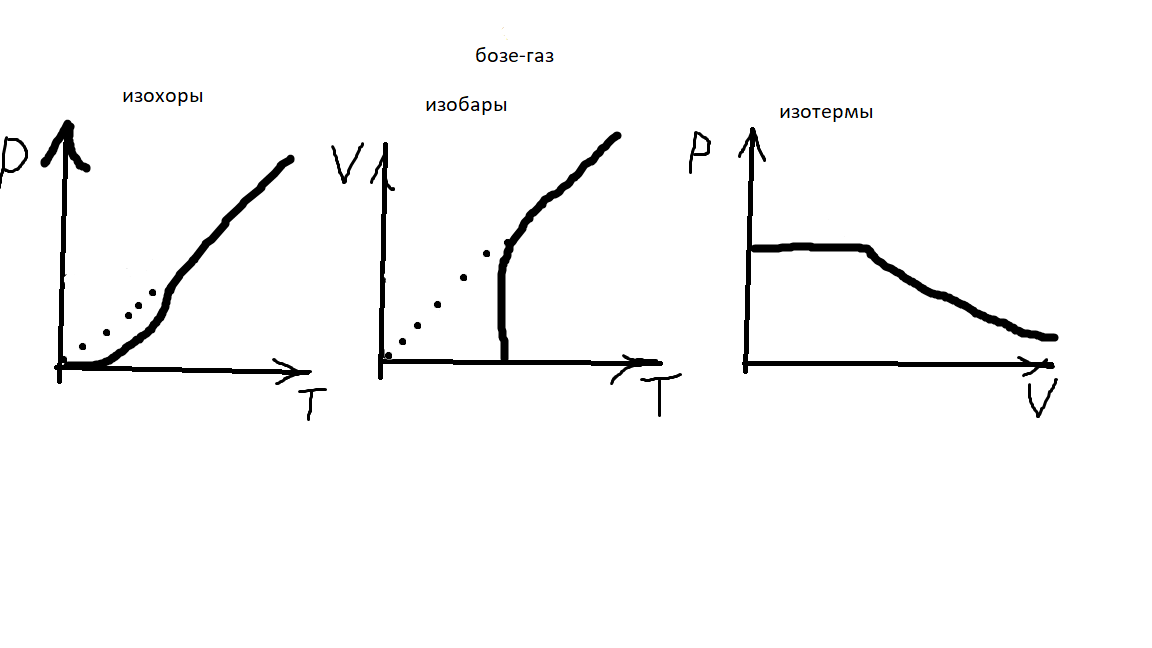
\includegraphics[width=0.7\linewidth]{bosegraphs}
	\caption{}
	\label{fig:fermigraphs}
\end{figure}





\end{ttask}


\begin{ttask}\textbf{12.} 
	
Построить изохоры, изобары и изотермы для ферми-газа. 

При $ T<<\varepsilon_{r} \quad p \approx \gamma\left(\frac{N}{v}\right)^{5 / 3} $




\begin{figure}[H]
	\centering
	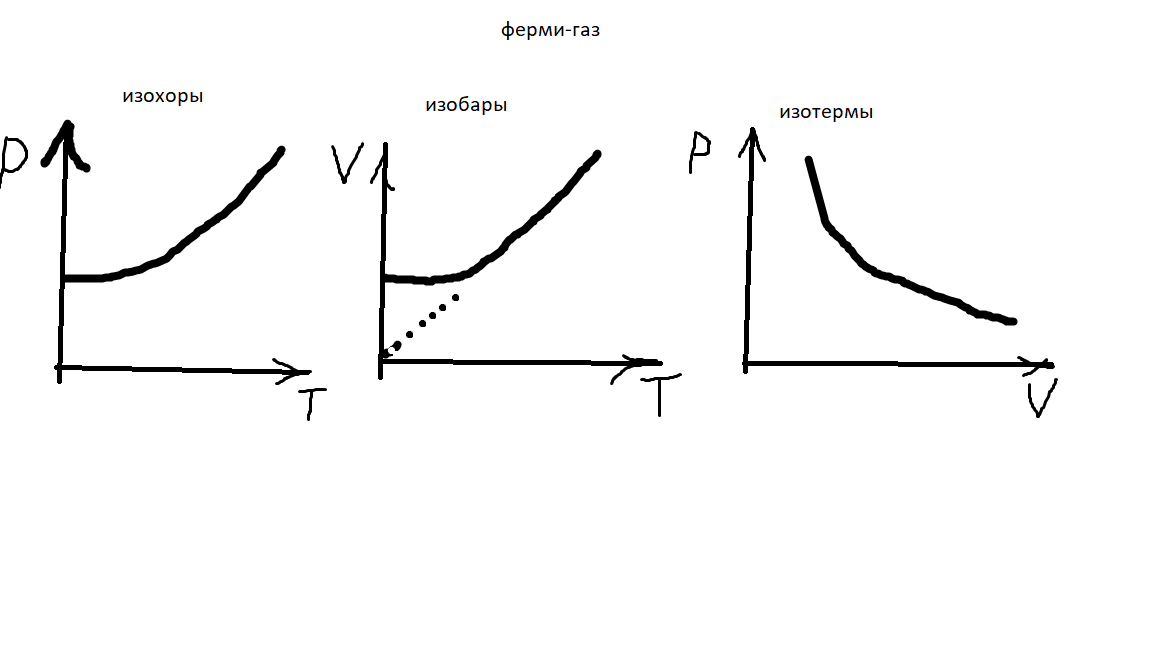
\includegraphics[width=0.7\linewidth]{fermi_graphs}
	\caption{}
	\label{fig:fermigraphs}
\end{figure}












\end{ttask}


\begin{ttask}\textbf{13.} 

Вычислить теплоемкость двумерного вырожденного идеального ферми-газа. 




\[ dN_p = g \bar{n}_p \frac{d p_x d p_y d V }{(2\pi \hbar)^2}=
\frac{g V p dp}{2\pi \hbar^2 \left(\exp \left(\frac{\varepsilon-\mu }{T}\right)+1 \right) }
 \]

\[\varepsilon=\frac{p^2}{2m} \Rightarrow  p dp=m d \varepsilon\]

\[ dN_\varepsilon= \left(\frac{g m }{2\pi \hbar^2}\right) V \frac{d \varepsilon }{e^{(\varepsilon-\mu)/T}+1}=
\left(\frac{g m }{2\pi \hbar^2}\right) V T \frac{dx}{e^{x-y}+1}
\]

\[ E= \left(\frac{g m }{2\pi \hbar^2}\right) V T^2 \int_{0}^{\infty}\frac{x dx}{e^{x-y}+1} \approx
\left(\frac{g m }{2\pi \hbar^2}\right) V T^2 \left(  \left(\frac{\mu^2}{2T^2}\right)+\frac{\pi^2}{6}\right)\]


\[ C=\frac{1}{V}\frac{dE}{dT}=
\left(  \frac{g m }{2\pi \hbar^2}\right)\frac{\pi^2}{3} T\]














\end{ttask}


\begin{ttask}\textbf{14}. 

Вычислить теплоемкость черного излучения. 



Химический потенциал
фотонного газа равен нулю. 

Распределение фотонов дается
соотношением:
\[ \bar{n}=\frac{1}{\operatorname{exp}\left(\frac{\hbar \omega_{k}}{T}\right)-1} \]

Число состояний определяется соотношением
$$
2 \frac{V 4 \pi k^{2} d k}{(2 \pi)^{3}}=2 \frac{V 4 \pi \omega_{k}^{2} d \omega_{k}}{(2 \pi c)^{3}}
$$

Дополнительный фактор 2 возникает из-за двух поляризаций фотонов.

Подставляя это число в $ \bar{N_{n}}$, получаем:
$$
d N_{\omega}=\frac{1}{\exp (\hbar \omega / T)-1} \frac{V \omega^{2} d \omega}{\pi^{2} c^{3}}
$$
Энергия излучения получается из $ d N_{\omega} $ умножением на энергию фотона
\begin{equation}\label{plank}
d E_{\omega}=
\frac{1}{\exp (\hbar \omega / T)-1} \frac{V \hbar \omega^{3} d \omega}{\pi^{2} c^{3}}
\end{equation}
Формула \ref{plank} - называется формулой Планка. 

Дальше считаем свободную энергию.
$$
	F=T \sum_{k} \ln \left[1-\exp \left(-\frac{\varepsilon_{k}}{T}\right)\right]
	=T \frac{V}{\pi^{2} c^{3}} \int_{0}^{\infty} \omega^{2} \ln \left[1-\exp \left(-\frac{\hbar \omega}{T}\right)\right] d \omega
$$
Заменяя переменную интегрирования $\quad x=\hbar \omega / T \quad$ и интегрируя по
частям, отсюда получим
$$
F=-\frac{V T^{4}}{3 \pi^{2} \hbar^{3} c^{3}} \int_{0}^{\infty} \frac{x^{2} d x}{\exp (x)-1}
$$
Безразмерный интеграл в этом соотношении равен $\pi^{4} / 15 .$ Итак, свободная энергия равна
$$
F=-\frac{\pi^{2} V T^{4}}{45 \hbar^{3} c^{3}}=-\frac{4 \sigma}{3 c} V T^{4}
$$


Коэффициент $\sigma$ называется постоянной Стефана-Больцмана:
$$
\sigma=\frac{\pi^{2} k^{4}}{60 \hbar^{3} c^{2}}=5.67 \cdot 10^{-5} \frac{\text{г}}{\text{сек}^{3}\text{град}^{4} }
$$
(если температура измеряется в градусах Кельвина). Зная свободную энергию, определяем обычную энергию (закон Больцмана)
$$
E=F-T\left(\frac{\partial F}{\partial T}\right)_{V}=\frac{4 \sigma}{c} V T^{4}
$$
Для теплоемкости излучения в полости с заданным объемом получаем
$$
C_{V}=\frac{16 \sigma}{c} V T^{3}
$$


















 

\end{ttask}


\begin{ttask}\textbf{15}

Найти равновесную плотность и теплоемкость акустических фононов в кристалле при температурах выше $ T $  и ниже $ T $  дебаевской




Гамильтониан атомов решётки кристалла может быть диагонализирован, 
т. е. разложен по нормальным модам колебаний. 
В представлении вторичного квантования он имеет вид



$$
	\hat{H}=\sum_{\mathbf{k}} \frac{1}{2}\left(\mathbf{p}_{\mathbf{k}}^{2}+\omega_{\mathbf{k}}^{2} \mathbf{q}_{\mathbf{k}}^{2}\right)=\sum_{\mathbf{k}, \text { З поляризац.}}  \hbar \omega_{\mathbf{k}}\left(\hat{a}_{\mathbf{k}}^{+} \hat{a}_{\mathbf{k}}+\frac{1}{2}\right)
$$
Где $\hat{a}_{\mathbf{k}}^{+}$ оператор рождения, $n_{\mathbf{k}}=\hat{a}_{\mathbf{k}}^{+} \hat{a}_{\mathbf{k}}-$ числа заполнения мод. 
Мы ограничимся рассмотрением только акустических мод колебаний $\omega_{\mathrm{k}}=v_{l, t} \cdot k,$ 
поскольку при низких температурах в системе возбуждаются состояния с минимальными частотами. 
У звука в кристалле есть две поперечные моды со скоростью звука $v_{t}$ и одна продольная со скоростью звука
$v_{l},$ так что плотность числа состояний
$$
g(\omega)=\frac{V \omega^{2} d \omega}{2 \pi^{2}}\left(\frac{1}{v_{l}^{3}}+\frac{2}{v_{t}^{3}}\right)
$$
которую для краткости мы будем записывать как
$$
g(\omega)=\frac{3}{2} \cdot \frac{\omega^{2} d \omega}{\pi^{2} v^{3}}
$$
введя эффективную скорость звука $v:$


$$
\frac{3}{v^{3}}=\frac{2}{v_{t}^{3}}+\frac{1}{v_{l}^{3}}
$$
Поскольку фононы являются возбуждениями не пустого пространства, а коллективными колебаниями «пустого» кристалла, 
состоящего из $N$ атомов, существует важное отличие их одночастичных состояний от фотонов. 
В $\mathbf{k}$ -пространстве фононные состояния занимают только конечную сферу Дебая с радиусом $k_{D}$. 
Действительно, число степеней свободы кристалла равно числу его атомов $3 N$, 
значит столько же «точек» одночастичных состояний должно быть в сфере Дебая:
$$
\frac{3 V}{2 \pi^{2} v^{3}} 
\cdot 
\int_{0}^{\omega_{D}} \omega^{2} d \omega
=3 N
$$
где частота Дебая есть
$$
\omega_{D}
=
c k_{D}
=
v\left(\frac{6 \pi^{2} N}{V}\right)^{1 / 3}
$$



Физический смысл этого ограничения ясен: длина волны фонона не может быть меньше 
постоянной решётки $a=(V / N)^{1 / 3},$ а его частота, соответ-
ственно, должна быть меньше дебаевской $\omega \leq 2 \pi v / a \sim \omega_{D} .$ 
Тогда энергия идеального газа фононов в этом приближении равна
$$
E(T)=\int_{0}^{\omega_{D}} \frac{3 V \omega^{2}}{2 \pi^{2} v^{3}} \cdot \frac{\hbar \omega}{e^{\frac{h \omega}{T}}-1} d \omega
=
\frac{3 V T^{4}}{2 \pi^{2} v^{3} \hbar^{3}} \cdot \int_{0}^{\Theta_{D} / T} \frac{x^{3} d x}{e^{x}-1}
$$
Энергия $E(T)$ существенно зависит от величины температуры Дебая:
$\Theta_{D}=\hbar \omega_{D} .$ 


При низких температурах $T \ll \Theta_{D}$ верхний предел интегрирования можно заменить на $\infty$, 
и фононный газ ведёт себя так же, как тепловое излучение. 
Для его теплоемкости получаем закон Дебая:
$$
C_{V}(T)=\frac{12 \pi^{4}}{5} N\left(\frac{T}{\Theta_{D}}\right)^{3} \propto T^{3}
$$




При высоких температурах $T \gg \Theta_{D}$ все состояния сферы Дебая заполнены, 
и мы получаем закон равнораспределения по степеням свободы Дюлонга-Пти:
$$
C_{V}=3 N
$$




\end{ttask}


\begin{ttask}\textbf{16}

Используя представление оператора смещения гармонического осциллятора 

$\hat{x}=\left(\frac{\hbar}{2 m \omega}\right)^{1 / 2}\left(\hat{b}^{+}+\hat{b}\right),$ 
получить формулу $\left\langle e^{i k \hat{x}}\right\rangle=$
$=e^{-\frac{k^{2} \hbar}{4 m \omega}}$ при температуре $T=0$

















\end{ttask}




\begin{ttask} \textbf{17}


Описать парамагнетизм Паули и диамагнетизм Ландау. 
Рассмотреть эффект де Гааза–ван Альфена в двумерном металле. 




Парамагнетизм.


Наиболее просто намагниченность вычисляется в высокотемпературном пределе $T \gg T_{\text {выр}}$. 
В высокотемпературном приближении электронный газ больцмановский, 
его статистическая сумма факторизуется и достаточно вычислить её для одной частицы в поле $\mathcal{B}.$ 

Парамагнетизм связан с наличием у электрона собственного магнитного момента $\mu_{B}=e \hbar / 2 m c,$ 
так что его энергия в поле есть $\pm \mu_{B} \mathcal{B} .$ 
Вводя для удобства $x=\mu_{B} \mathcal{B} / T,$ получаем в расчете на один электрон
$$
\begin{array}{c}
	z=e^{-\frac{\mu_{B} B}{T}}+e^{\frac{\mu_{B} B}{T}}=2 \operatorname{ch} x 
	\\
	f=-T \ln z
	=
	-T \ln (2 \operatorname{ch} x) 
	\\
	m=-\left(\frac{\partial f}{\partial \mathcal{B}}\right)
	=
	\mu_{B} \frac{\partial}{\partial x} \ln (2 \operatorname{ch} x)
	=
	\mu_{B} \operatorname{th} x
\end{array}
$$
Полученная формула (8.6) имеет ясный физический смысл. 
В нулевом поле температура «размешивает» моменты электронов по направлениям, 
и магнитный момент газа отсутствует. 
При небольших полях $\mu_{B} \mathcal{B} \ll T$ наведённый магнитный момент линеен по полю, и удобно ввести


Восприимчивость $\chi$ в расчете на одну частицу определяется как 
$\chi=\lim _{\mathcal{B} \rightarrow 0} m / \mathcal{B} .$ 

Поэтому получаем $\chi=\mu_{B}^{2} / T .$

Эта зависимость называется законом Кюри и показывает, что при больших температурах магнетизм исчезает.






Кроме положительной парамагнитной восприимчивости, существует еще 
отрицательная диамагнитная восприимчивость. 

Диамагнетизм возникает из-за дискретности уровней Ландау энергии электронов $\varepsilon_{n}=\hbar \omega(n+1 / 2)$
кратностью $\quad$ вырождения $ g_{L}=\mathcal{B} S / \Phi_{0}$. 

Здесь $\hbar \omega=2 \mu_{B} \mathcal{B}-$ циклотронная частота, 
а $\Phi_{0}=2 \pi \hbar c / e-$ квант потока, так
что кратность вырождения уровня Ландау $g_{L}$ - это просто число квантов
потока $\Phi / \Phi_{0}$, проходящего через поперечное к полю сечение образца. В
этом случае одночастичная статсумма равна
$$
z
=
g_{L} \sum_{n=0}^{\infty} 
e^{-\frac{h \omega}{T}\left(n+\frac{1}{2}\right)}
=
\frac{g_{L}}{2 \operatorname{sh} x}
$$
где учтено, что $x=\hbar \omega / 2 T=\mu_{B}$ В $/ T$. Отсюда в расчете на один электрон
получаем
$$
\begin{array}{c}
	f=-T \ln z=-T \ln \frac{x}{\operatorname{sh} x}+\ldots 
	\\
	m=-\left(\frac{\partial f}{\partial \mathcal{B}}\right)
	=
	\mu_{B} \frac{\partial}{\partial x} \ln \frac{x}{\operatorname{sh} x}
	=
	-\mu_{B}\left(\operatorname{cth} x-\frac{1}{x}\right)
\end{array}
$$


Намагниченность описывается функцией Ланжевена: $m=-\mu_{B} \mathcal{L}(x),$ 
а диамагнитная восприимчивость
$$
\chi_{\text {диа }}=\left(\frac{\partial m}{\partial \mathcal{B}}\right)_{B=0}=-\frac{\mu_{B}^{2}}{3 T}
$$
в три раза меньше парамагнитной $\chi_{\text {диа}}=-\chi_{\text {пара}} / 3 .$ Таким образом, в целом
электронный газ парамагнитен: $\chi_{\text {диа}}+\chi_{\text {пара}}>0 .$



Если зеемановская энергия электронов становится больше температуры $T<\mu_{B} \mathcal{B} \ll \varepsilon_{F},$ то магнитное поле называют «квантующим». 
В этих условиях становится существенной дискретность уровней Ландау, что приводит к 
появлению у намагниченности электронного газа осциллирующей части. 
Амплитуда этих осцилляций не мала, а «шаг» осцилляций по обратному магнитному полю постоянен. 
Это доставляет ценную информацию о свойствах ферми-поверхности металла. Поэтому эффект заслужил имя собственное, де Гааза-ван Альфрена (1930). 
Для того, чтобы оценить амплитуду и «шаг» по полю осцилляций де Гааза-ван Альфена, 
рассмотрим самый простой случай: двумерный ( $\mathrm{D}=2$ ) электронный газ при нулевой температуре $(T=0) .$ Тогда в 
магнитном поле $N$ электронов газа распределены по уровням Ландау следующим образом. 
На уровнях $0,1,2, \ldots, j$ «сидит» по $g_{L}$ электронов, а на последнем $j+1$ -м уровне - оставшиеся $N-g_{L}(j+1)$ штук. 
Таким будет распределение электронов в интервале значений приложенного поля:
$$
\frac{(j+1)}{B_{0}}<\frac{1}{B}<\frac{(j+2)}{B_{0}}
$$
где $\mathcal{B}_{0}=N \Phi_{0} / 2 S, S-$ площадь образца, $g_{L}=2 B S / \Phi_{0}-$ кратность вырождения уровня Ландау с учетом спина. 


Вычислим энергию основного состояния газа при $T=0$ :
$$
\begin{array}{l}
	E=g_{L} \sum_{k=0}^{j} 
	\hbar \omega
	\left(k+\frac{1}{2}\right)
	+
	\hbar \omega
	\left(j+\frac{3}{2}\right)
	\left(N-g_{L}(j+1)\right)
	= \\
	=
	2 N \mu_{B}
	\left[
	\frac{B}{B_{0}}\left(j+\frac{3}{2}\right)
	-
	\left(\frac{\mathcal{B}}{B_{0}}\right)^{2}(j+1)\left(\frac{j}{2}+1\right)
	\right]
\end{array}
$$
При нулевой температуре свободная энергия совпадает с внутренней $F=E-T S$. 
Магнитный момент $M=-\partial E / \partial \mathcal{B}$ основного состояния 
электронного газа при нулевой температуре в указанном интервале полей равен
$$
M(\mathcal{B})
=
N \cdot \frac{e \hbar}{m c} \cdot
\left[
(j+1)(j+2) \frac{\mathcal{B}}{\mathcal{B}_{0}}
-
j-\frac{3}{2}
\right]
$$



При изменении магнитного поля последний уровень Ландау постепенно заполняется, пока число $j$ скачком не увеличится на единицу. В следующем
по $j \rightarrow j+1$ интервале обратных полей повторяется точно такая же зависимость $M(\mathcal{B})$. 
Таким образом, магнитный момент $M$ осциллирует в интервале $\pm N \mu_{B}$ с постоянным по обратному полю шагом:
$$
\frac{1}{\mathcal{B}_{0}}=\frac{e S}{\pi \hbar c N}=\frac{\mu_{B}}{\varepsilon_{F}}
$$
Физический смысл осцилляций намагниченности связан с периодическим заполнением и 
опорожнением последнего по счёту заполняемого уровня Ландау. 
Чтобы эти осцилляции были выражены и не «размывались» температурными эффектами, необходимо, 
чтобы поле было квантующим $T \ll \mu_{B} \mathcal{B},$ а 
электронный газ вырожденным $\mu_{B} \mathcal{B} \ll \varepsilon_{F} .$ 






























\end{ttask}


\begin{ttask}\textbf{18. }

Сравнить низкотемпературные зависимости теплоемкости идеальных бозе- и ферми-газов, 
черного излучения и твердого тела, 
парамагнетика и ферромагнетика, 
неидеального бозе-газа и, наконец, сверхпроводника. 



Вырожденные ферми- и бозе-газы $\left(T \ll T_{\text {выр}}\right)$ ведут себя очень по-
разному. 

Рассмотрим сначала ферми-газ. 

Запишем, как и ранее, выражение для энергии:
$$
E=B V \cdot \int_{0}^{\infty} 
\frac{\sqrt{\varepsilon} \cdot \varepsilon d \varepsilon}{e^{\frac{\varepsilon-\mu}{T}}+1}
$$
Низкотемпературные свойства фермионов определяются тем, 
что при $T=0$ сфера Ферми заполнена, а при увеличении температуры заполненность состояний изменяется 
в узком слое шириной $\sim T$ около поверхности Ферми. 
Как отмечалось выше, при $T \ll T_{\text {выр}}$ функция распределения Ферми-Дирака 
имеет вид резко выраженной «ступеньки», так что, полагая в $\mu=\mu(0),$ получаем
$$
E=
\frac{2}{5} B V \mu^{5 / 2}(0)
=
\frac{3}{2}PV
$$


Чтобы вычислить теплоёмкость вырожденного ферми-газа, 
нужно «выделить» отличие функции распределения Ферми-Дирака от «ступеньки». 
Это отличие мало в меру малости $T / \varepsilon_{F} \ll 1,$ то есть наш интеграл нужно разложить по этому малому параметру:

$$
\int_{0}^{\infty} \frac{f(\varepsilon) d \varepsilon}{e^{\frac{\varepsilon-\mu}{T}}+1}=\int_{0}^{\mu} f(\varepsilon) d \varepsilon+\frac{\pi^{2}}{6} T^{2} f^{\prime}(\mu)+\ldots
$$

Тогда
$$
E=\frac{2}{5} B V \mu^{5 / 2}
\left[
1
+
\frac{5 \pi^{2}}{8}\left(\frac{T}{\mu}\right)^{2}
+
\ldots
\right]
$$


Тогда


\[ C_{V}(T)=\frac{\pi^{2}}{2} \cdot N \cdot \frac{T}{\varepsilon_{F}}+\ldots \]



Здесь учтено, что  $2 B V \mu^{5 / 2}(0) / 5=3 N \varepsilon_{F} / 5$. 

Линейная зависимость теплоемкости от температуры имеет ясный физический смысл. 
При нулевой температуре сфера Ферми полностью заполнена. 
При нагревании газа до небольшой температуры $T$ происходит изменение чисел электронов только в узком слое $\sim T$ вблизи поверхности Ферми. 
Относительная доля электронов, переместившихся в возбужденные состояния, $\sim T / \varepsilon_{F}$, а изменение энергии каждого $\sim T$, 
так что теплоёмкость газа получается $C_{V} \sim N T / \varepsilon_{F}$.






Теперь вычислим теплоемкость бозе-газа, для этого найдем энергию. 
Поскольку $\varepsilon_{0}=0$ при $\mathbf{p}=0$ и $T<T_{B}$ получаем
$$
E=B V T^{5 / 2} \cdot \int_{0}^{\infty} \frac{x^{3 / 2} d x}{e^{x}-1}
$$
Здесь безразмерный интеграл в численно равен 1.78 , так что
$$
E \approx 0.77 \cdot N T\left(\frac{T}{T_{B}}\right)^{5 / 2}
$$
а теплоёмкость равна
$$
C_{V}
=
\frac{\partial E}{\partial T} 
\approx 
1.92 \cdot N\left(\frac{T}{T_{B}}\right)^{3 / 2} 
\propto 
T^{3 / 2}
$$




А для черного тела теплоемкость была найдена в задаче 14:
$$
C_{V}=\frac{16 \sigma}{c} V T^{3}
$$





Для теплоемкости твердого тела известен закон Дебая:
$$
C_{V}(T)=\frac{12 \pi^{4}}{5} N\left(\frac{T}{\Theta_{D}}\right)^{3} \propto T^{3}
$$



Для сверхпроводника по лекциям было получено выражение:

Тогда теплоемкость
$$
C_{s}
=
C_{n}+\frac{T_{c}}{2 A} \nu(0)
$$
то есть всё линейно, только при переходе в сверхпроводящее состояние имеется скачок.




теплоемкости диа и пара магнетиков определяются свойствами твердого тела и вкладом электронов, 
а это было уже описано выше.











\end{ttask}






\begin{ttask} \textbf{19.}
	 
Показать, что фазовая скорость элементарного возбуждения в бозе-конденсате равна гидродинамической скорости звука.


















\end{ttask}



\begin{ttask} \textbf{20}

Найти распределение частиц по импульсам и полное число надконденсатных частиц в идеальном и неидеальном бозе-газах при T = 0 и низких температурах.





В случае идеального бозе-газа число надкондексатных частиц известно:
\[ N_{0}=N\left[1-\left(\frac{T}{T_{c}}\right)^{3 / 2}\right] 
\]

Получим его:


Полное число частиц
$$
N=\sum_{p} N_{p}=\sum_{p} \frac{1}{e^{\beta\left(\varepsilon_{p}-\mu\right)}-1}
$$
не зависит от температуры и, тем самым неявным образом залает зависимость химического потенциала от температуры. 

Преобразуем его с помощью правила Бора-Зоммерфельда, согласно которому для любой функции 
от энергии сумма по импульсам эквивалентна интегралу
$$
I=
\sum_{p} f\left(\varepsilon_{p}\right)=
\int \frac{L^{3} d^{3} p}{(2 \pi \hbar)^{3}} f\left(\varepsilon_{p}\right)=
\nu V \int_{0}^{\infty} \varepsilon^{1 / 2} d \varepsilon f(\varepsilon)
$$
где $\nu=\frac{m^{3 / 2}}{2^{1 / 2} \pi^{2} \hbar^{3}} .$ 


Поэтому, переобозначив $z=p^{2} / 2 m T$, полное число частиц станет
$$
N=T^{3 / 2} \nu V \int_{0}^{\infty} \frac{z^{1 / 2} d z}{e^{z} e^{-\beta \mu}-1}.
$$


Исследуем это выражение для поиска $ \mu(T) $. 
Запишем его в виде:
$$
\int_{0}^{\infty} \frac{z^{1 / 2} d z}{e^{z} e^{-\beta \mu}-1}=\frac{N}{T^{3 / 2} \nu V}
$$
Чтобы при росте температуры интеграл падал как $T^{-3 / 2},$ необходимо падение подынтегрального выражения, 
т.е. член $e^{z-\beta \mu}$ должен расти с $z$.
Поэтому при достаточно высоких температурах единицей в 
подынтегральном выражении можно пренебречь и, считая $ \mu(T)\ne \mu(z)$ (????), 
запишем равенство через гамма функцию:
%
$$
N=\Gamma(3 / 2) T^{3 / 2} \nu V e^{\beta \mu},
$$
поэтому $e^{\beta \mu} \sim T^{3 / 2}$ и видим понижение химического потенциала по закону
$$
\mu \sim-\frac{3}{2} T \ln \frac{1}{T}
$$

И видим, что при больших температурах в знаменателе распределения Бозе-Эйнштейна можно пренебречь единицей и перевести 
распределение Бозе в распределение Максвелла-Больцмана
$$
N_{p}=e^{\beta\left(\mu-\varepsilon_{p}\right)}
$$


А если дальше понижать температуру, то уже невозможно, чтобы выполнялось исследуемое уравнение, 
потому что уже стабильно $\mu=0 .$ 
А так как мы его получили из правила Бора-Зоммерфельда, то понятно, что нужно как-то иначе его применить.
Так как в области низких температур число частиц на нижнем уровне $N_{0}$ очень велико, 
то следует заменять сумму на интеграл только для возбужденных состояний плюс число частиц на нулевом уровне
$$
N=\sum_{p} N_{p}
=
N_{0}+T^{3 / 2} \nu V 
\int_{0}^{\infty} d z 
\frac{z^{1 / 2}}{e^{z}-1}
$$


В итоге выражаем находим температурную зависимость числа $N_{0}:$
$$
N_{0}=N\left[1-\left(\frac{T}{T_{c}}\right)^{3 / 2}\right]
$$





Рассмотрим неидеальный бозе-газ



Из преобразований Боголюбова следует, что среднее по состоянию газа число частиц с импульсом $k$ равно
$$
N_{k}=\left\langle\hat{a}_{k}^{+} \hat{a}_{k}\right\rangle=v_{k}^{2}+u_{k}^{2}\left\langle\hat{b}_{k}^{+} \hat{b}_{k}\right\rangle+v_{k}^{2}\left\langle\hat{b}_{-k}^{+} \hat{b}_{-k}\right\rangle
$$
При нулевой температуре квазичастицы отсутствуют, и первый член здесь дает
$$
N_{k}^{(0)}
=
v_{k}^{2}
=
\frac{1}{2}\left(
\frac{\xi_{k}}{\varepsilon_{k}}-1
\right)
$$
При $\varepsilon_{k} \ll \mu$ это число весьма велико, но при $\varepsilon_{k} \gg \mu$ быстро падает. 
Полное число надконденсатных частиц по порядку величины равно, очевидно, 
числу состояний свободных частиц с импульсами меньше $p_{\max }=\sqrt{2 m \mu} .$ 
Это число равно
$$
n_{1}^{(0)}
=
\frac{1}{V} \sum N_{k}^{(0)} 
\simeq 
\frac{p_{\max }^{3}}{(2 \pi \hbar)^{3}} 
\simeq 
n_{0} \sqrt{n_{0} a^{3}}
$$
Теория Боголюбова опирается на предположение, 
что в основном состоянии большинство частиц находится в конденсате, и $n_{1}^{(0)} \ll n_{0} .$ 


Отсюда находим оценку максимальной плотности газа
\[ \max n_{0} \simeq a^{-3} \]


В зависимости от рассматриваемой области температур плотность возбужденных частиц по порядку величины равна



$$
\begin{aligned}
	n_{1}^{(T)} & \simeq \frac{\mu}{T}\left(\frac{T}{c}\right)^{3}, 0<T<\mu \\
	n_{1}^{(T)} & \simeq \sum N_{k} \simeq(m T)^{3 / 2}, \mu<T \ll T_{c} \frac{\mu}{T_{c}}=a n^{1 / 3}
\end{aligned}
$$
Подчеркнем, что энтропия конденсата равна нулю, и при $T \ll T_{c}$ вклад в энтропию и теплоемкость дают только надконденсатные частицы.






\end{ttask}



\begin{ttask} \textbf{21}

Определить свободную энергию одномерной цепочки спинов 1/2 с гамильтонианом

$$\hat{H}
=
-J \sum_{k}^{N} \hat{\sigma}_{k}^{z} \hat{\sigma}_{k+1}^{z}, \quad \hat{\sigma}_{N+1}^{z}
=
\hat{\sigma}_{1}^{z}$$
Вычислить теплоёмкость и объяснить причину отсутствия фазового перехода при $ T\ne 0 $




статсумма запишется
$$
Z_{N}=
\sum_{\sigma_{1}=\pm 1} \ldots \sum_{\sigma_{N}=\pm 1} 
\exp 
\left(K \sum_{j=1}^{N-1} \sigma_{j} \sigma_{j+1}\right), 
\quad
K=J / T
$$


Представим её в виде
$$
Z_{N}=\sum_{\sigma_{1}=\pm 1} \ldots \sum_{\sigma_{N-1}=\pm 1} \exp \left(K \sum_{j=1}^{N-2} \sigma_{j} \sigma_{j+1}\right) \sum_{\sigma_{N}=\pm 1} \exp \left(K \sigma_{N-1} \sigma_{N}\right)
$$
Поскольку 
$\sum_{\sigma_{N}=\pm 1} 
\exp \left(K \sigma_{N-1} \sigma_{N}\right)
=2  ch K,$ 
то
$$
Z_{N}=Z_{N-1}(2 c h K)=Z_{2}(2 c h K)^{N-2}
$$



Ho
$$
Z_{2}=\sum_{\sigma_{1}=\pm 1} \sum_{\sigma_{2}=\pm 1} \exp \left(K \sigma_{1} \sigma_{2}\right)=4 \operatorname{ch} K
$$

поэтому
$$
Z_{N}=2(2 c h K)^{N-1}
$$



Свободная энергия имеет вид
$$
F=-T \ln Z=-N T \ln (2 c h K)
$$




Соответственно энергия и теплоемкость имеют вид
$$
\begin{aligned}
	E &=\frac{\partial}{\partial \frac{1}{T}}\left(\frac{F}{T}\right)=-N J t h \frac{J}{T} \\
	C &=\frac{\partial E}{\partial T}=\frac{N J^{2} / T^{2}}{c h^{2} \frac{J}{T}}
\end{aligned}
$$
В пределе высоких и низких температур $C \rightarrow 0 .$







\end{ttask}



\begin{ttask}

22. Для ферромагнетика в модели Гейзенберга при $ T \ll T_c $ определить спектр возбуждений (магнонов) и найти температурную зависимость намагниченности и теплоемкости спиновых волн.

















\end{ttask}



\begin{ttask}

23. Для ферромагнетика в модели Гейзенберга в приближении самосогласованного поля определить температуру Кюри Tc, 
температурную зависимость магнитной восприимчивости  и спонтанной намагниченности вблизи Tc. 
Сравнить с результатами теории Ландау.





















\end{ttask}



\begin{ttask}  \textbf{24}

Определить корреляционный радиус флуктуации параметра порядка в нулевом внешнем поле вблизи точки фазового перехода II рода. 

Найти флуктуационную поправку к теплоемкости при $ T = T_c $ в теории Гинзбурга–Ландау.



















\end{ttask}





\begin{ttask}

25. Доказать, что плотность сверхтекучей компоненты электронного газа при T = 0 равна полной плотности числа частиц.  

















\end{ttask}






\begin{ttask} \textbf{26.} 

В модели БКШ определить скачок теплоемкости.



Тепловые свойства сверхпроводника определяются его возбужениями - квазичастицами, 
которые можно рассматривать как ферми-газ с нулевым химическим потенциалом. 
Энтропия этого газа равна
$$
S=-\sum[n \ln n+(1-n) \ln (1-n)]
$$

здесь 
$n=\left(e^{\beta \varepsilon}+1\right)^{-1}$,  
$\varepsilon=\sqrt{\xi^{2}+\Delta^{2}} $


Теплоемкость дается формулой из термодинамики:
$$
C=T \frac{\partial S}{\partial T}=\sum T \frac{\partial S}{\partial n} \frac{\partial n}{\partial T}=-\sum T[\ln n-\ln (1-n)] \frac{\partial n}{\partial T}
$$

$$
\ln n-\ln (1-n)=\ln \frac{n}{1-n}=-\ln \left(\frac{1}{n}-1\right)=-\beta \varepsilon
$$


Таким образом
$$
C=\sum \varepsilon \frac{\partial n}{\partial T}
$$
При низких температурах теплоемкость экспоненциально мала. 

Вблизи критической температуры самое сложное - 
найти производную от распределения квазичастиц
$$
\frac{\partial n}{\partial T}
=
\frac{\partial n}{\partial \beta \varepsilon} 
\frac{\partial \beta \varepsilon}{\partial T}
=
T \frac{\partial n}{\partial \varepsilon}
\left(-\frac{\varepsilon}{T^{2}}
+
\frac{1}{T} \frac{1}{2 \varepsilon} 
\frac{\partial \Delta^{2}}{\partial T}
\right)
$$
Квадрат пели линейно зависит от температуры
$$
\frac{\partial \Delta^{2}}{\partial T}=\frac{\partial}{\partial T} T_{c} \frac{T_{c}-T}{A}=-\frac{T_{c}}{A}
$$

Тогда теплоемкость
$$
C_{s}
=
\sum\left|\frac{\partial n}{\partial \varepsilon}\right|\left(\frac{\varepsilon^{2}}{T}+\frac{T_{c}}{2 A}\right)
=
C_{n}+\frac{T_{c}}{2 A} \sum\left|\frac{\partial n}{\partial \varepsilon}\right|
=
C_{n}+\frac{T_{c}}{2 A} \nu(0)
$$


Так как $C_{n}=\frac{\pi^{2}}{3} \nu(0) T$, 
то скачек теплоемкости в точке фазового перехода равен
$$
\frac{C_{s}-C_{n}}{C_{n}}=\frac{T_{c} \nu(0)}{2 A \frac{\pi^{2}}{3} \nu(0) T}=\frac{3}{2 A \pi^{2}}=1,43
$$














\end{ttask}

\begin{ttask}

27. Диагонализуя гамильтониан для фотонов и экситонов с учетом гибридизации, получить спектр поляритонов. 


(Преподаватель эту задачу убрал)












\end{ttask}



\begin{ttask}

28. Мешок Нагаоки (спиновый полярон большого радиуса в антиферромагнетике)

(Преподаватель эту задачу убрал)





\end{ttask}





\end{document}
